% rubber: rules rules.ini
% This is "sig-alternate.tex" V2.0 May 2012
% This file should be compiled with V2.5 of "sig-alternate.cls" May 2012
%
% This example file demonstrates the use of the 'sig-alternate.cls'
% V2.5 LaTeX2e document class file. It is for those submitting
% articles to ACM Conference Proceedings WHO DO NOT WISH TO
% STRICTLY ADHERE TO THE SIGS (PUBS-BOARD-ENDORSED) STYLE.
% The 'sig-alternate.cls' file will produce a similar-looking,
% albeit, 'tighter' paper resulting in, invariably, fewer pages.
%
% ----------------------------------------------------------------------------------------------------------------
% This .tex file (and associated .cls V2.5) produces:
%       1) The Permission Statement
%       2) The Conference (location) Info information
%       3) The Copyright Line with ACM data
%       4) NO page numbers
%
% as against the acm_proc_article-sp.cls file which
% DOES NOT produce 1) thru' 3) above.
%
% Using 'sig-alternate.cls' you have control, however, from within
% the source .tex file, over both the CopyrightYear
% (defaulted to 200X) and the ACM Copyright Data
% (defaulted to X-XXXXX-XX-X/XX/XX).
% e.g.
% \CopyrightYear{2007} will cause 2007 to appear in the copyright line.
% \crdata{0-12345-67-8/90/12} will cause 0-12345-67-8/90/12 to appear in the copyright line.
%
% ---------------------------------------------------------------------------------------------------------------
% This .tex source is an example which *does* use
% the .bib file (from which the .bbl file % is produced).
% REMEMBER HOWEVER: After having produced the .bbl file,
% and prior to final submission, you *NEED* to 'insert'
% your .bbl file into your source .tex file so as to provide
% ONE 'self-contained' source file.
%
% ================= IF YOU HAVE QUESTIONS =======================
% Questions regarding the SIGS styles, SIGS policies and
% procedures, Conferences etc. should be sent to
% Adrienne Griscti (griscti@acm.org)
%
% Technical questions _only_ to
% Gerald Murray (murray@hq.acm.org)
% ===============================================================
%
% For tracking purposes - this is V2.0 - May 2012
\pdfminorversion=4
\documentclass{sig-alternate}
\usepackage{caption}
\DeclareCaptionType{copyrightbox}
\graphicspath{{./figures/}}
\usepackage{subcaption}
\usepackage{url}
\usepackage{graphicx}
\usepackage{epstopdf}
\usepackage{multirow}
\usepackage{amsmath, amsfonts, amssymb}
\graphicspath{{./figures/}}
\usepackage{color}
%package for proper unicode rendering
\usepackage[utf8]{inputenc}
\usepackage{url}
\inputencoding{utf8}

\begin{document}
\newcommand{\narenc}[1]{[{\color{red} Naren writes: \it #1}]}
\newcommand{\sathappanc}[1]{[{\color{blue} Sathappan writes: \it #1}]}
%\newcommand{\grahamc}[1]{[\color{green} Graham writes: \it #1}]}
%symbols for psl rules 
\newcommand{\then}{\Rightarrow}
\newcommand{\softor}{\operatornamewithlimits{\tilde{\vee}}}
\newcommand{\softand}{\operatornamewithlimits{\tilde{\wedge}}}
\newcommand{\softthen}{\operatornamewithlimits{\tilde{\then}}}
\newcommand{\softneg}{\operatornamewithlimits{\tilde{\neg}}}



%
% --- Author Metadata here ---
%\conferenceinfo{WOODSTOCK}{'97 El Paso, Texas USA}
%\CopyrightYear{2007} % Allows default copyright year (20XX) to be over-ridden - IF NEED BE.
%\crdata{0-12345-67-8/90/01}  % Allows default copyright data (0-89791-88-6/97/05) to be over-ridden - IF NEED BE.
% --- End of Author Metadata ---

\title{Forecasting Protests \\by Detecting Future Time Mentions \\in News and Social Media}
%\subtitle{[Extended Abstract]
%\titlenote{A full version of this paper is available as
%\textit{Author's Guide to Preparing ACM SIG Proceedings Using
%\LaTeX$2_\epsilon$\ and BibTeX} at
%\texttt{www.acm.org/eaddress.htm}}}
%
% You need the command \numberofauthors to handle the 'placement
% and alignment' of the authors beneath the title.
%
% For aesthetic reasons, we recommend 'three authors at a time'
% i.e. three 'name/affiliation blocks' be placed beneath the title.
%
% NOTE: You are NOT restricted in how many 'rows' of
% "name/affiliations" may appear. We just ask that you restrict
% the number of 'columns' to three.
%
% Because of the available 'opening page real-estate'
% we ask you to refrain from putting more than six authors
% (two rows with three columns) beneath the article title.
% More than six makes the first-page appear very cluttered indeed.
%
% Use the \alignauthor commands to handle the names
% and affiliations for an 'aesthetic maximum' of six authors.
% Add names, affiliations, addresses for
% the seventh etc. author(s) as the argument for the
% \additionalauthors command.
% These 'additional authors' will be output/set for you
% without further effort on your part as the last section in
% the body of your article BEFORE References or any Appendices.
%\numberofauthors{6}
\numberofauthors{2}

\author{
% 1st. author
%\alignauthor
%Sathappan Muthiah\\
%       \affaddr{Virginia Tech, Blacksburg, VA 24061}\\
%       \email{sathap1@cs.vt.edu}
%% 2nd. author
%\alignauthor
%Bert Huang\\
%       \affaddr{University of Maryland, College Park, MD 20742}\\
%       \email{bert@cs.umd.edu}
%% 3rd. author
%\alignauthor
%Jaime Arredondo\\
%       \affaddr{University of California at San Diego, San Diego, CA 92093}\\
%       \email{jarredon@ucsd.edu}
%\and  % use '\and' if you need 'another row' of author names
%% 4th. author
%\alignauthor
%David Mares\\
%       \affaddr{University of California at San Diego, San Diego, CA 92093}\\
%       \email{dmares@ucsd.edu}
%% 5th. author
%\alignauthor
%Lise Getoor\\
%       \affaddr{University of California at Santa Cruz, Santa Cruz, CA 95064}\\
%       \email{getoor@soe.ucsc.edu}
%% 6th. author
%\alignauthor
%Graham Katz\\
%       \affaddr{CACI Inc., Lanham, MD 20706}\\
%       \email{ekatz@caci.com}
%\and
%% 7th. author
%\alignauthor
%Naren Ramakrishnan\\
%       \affaddr{Virginia Tech, Blacksburg, VA 24061}\\
%       \email{naren@cs.vt.edu}
}
\maketitle
\begin{abstract}
Civil unrest events (protests, strikes, and ``occupy'' events) are common occurrence in both democracies and authoritarian regimes. The study of civil unrest is a key topic for political scientists as it helps capture an important mechanism by which citizenry express themselves. In countries where civil unrest is lawful, qualitative analysis has revealed that more than 75\% of the protests are planned, organized, and/or announced in advance; therefore detecting future time mentions in relevant news and social media is a direct way to develop a protest forecasting system. We develop such a system in this paper, using a combination of key phrase learning to identify what to look for, probabilistic soft logic to reason about location occurrences in extracted results, and time normalization to resolve future tense mentions. We illustrate the application of our system to 10 countries in Latin America, viz. Argentina, Brazil, Chile, Colombia, Ecuador, El Salvador, Mexico, Paraguay, Uruguay, and Venezuela. Results demonstrate our successes in capturing significant societal unrest in these countries with an average lead time of 4.08 days. We also study the selective superiorities of news media versus social media (Twitter, Facebook) to identify relevant tradeoffs.

\end{abstract}

\iffalse
% A category with the (minimum) three required fields
\category{H.4}{Information Systems Applications}{Miscellaneous}
%A category including the fourth, optional field follows...
\category{D.2.8}{Software Engineering}{Metrics}[complexity measures, performance measures]
\terms{Theory}
\keywords{ACM proceedings, \LaTeX, text tagging}
\fi

\section{Introduction}
\label{intro}
Civil unrest (protests, strikes, and ``occupy'' events) is a common happening in both democracies
and authoritarian regimes.
Although we typically associate civil unrest with disruptions and instability, for a social scientist
civil unrest reflects the democratic process by 
which citizenry communicate their views and preferences to those in authority. 
The advent of social
media has afforded citizenry new mechanisms for organization and mobilization, and online news sources
and social networking sites like Facebook and Twitter
can provide a window into civil unrest happenings in a particular country.

Our basic hypothesis is that
protests that are larger will be more disruptive and communicate support for its cause better than smaller protests. 
Mobilizing large numbers of people is more likely to occur if a protest is organized and the time and place announced in
advance. Because protest is costly and more likely to succeed if it is large, we should expect planned, rather than 
spontaneous, protests to be the norm. Indeed, in a sample of 288 events from our study selected for qualitative review of their antecedents
(more details later), for 225 we located communications regarding the upcoming occurrence of the event in media, and only 49 were classified as 
spontaneous (we could not determine whether communications had or had not occurred in the remaining 14 cases).

Our goal here thus is to develop a protest forecasting system by identifying and mining mentions of future planned events
in (news and social) media. Why is this problem difficult? Consider the following situation:
\begin{quote}
An article is published in {\it El Universal}
in {\it Caracas, Venezuela} about a protest that happened over the {\it Friendship bridge} in {\it Foz do Iguacu, Brazil} due to
some conflict with citizens of {\it Paraguay}
across the border.
\end{quote}


We sought to develop
computational techniques for detecting overt direct indicators
of upcoming planned civil unrest events automatically from openly
available sources of information.  Detecting indicators for civil
unrest planning activities might have application to a wide range of
governmental and civil activity, from the issuance of travel warnings
to rapid emergency response capabilities.  
Our detection approach 
combine shallow linguistic analysis to identify a corpus of relevant
documents (articles, tweets) which are then subject to targeted deep semantic analysis.
Despite its simplicity, we are able to
detect indicators of event planning with surprisingly high
accuracy. 
Our contributions are:
\begin{enumerate}
\item We present a protest forecasting system that couples three key technical ideas:
key phrase learning to identify what to look for, probabilistic soft logic to reason about location occurrences in extracted results, and 
time normalization to resolve future tense mentions. We demonstrate how the integration of these ideas achieves objectives in precision,
recall, and quality (accuracy).
\item We illustrate the application of our system to 10 countries in Latin America, viz. Argentina, Brazil, Chile, Colombia, Ecuador, El Salvador, Mexico, Paraguay, Uruguay, and Venezuela. 
We conduct ablation studies to identify the 
relative contributions of news media (news + blogs) versus social media (Twitter, Facebook) to identify future happenings of
civil unrest. Through these studies we illustrate the selective superiorities of different sources for specific countries.
\narenc{Graham said to give some numerical values here.}
\item Unlike many studies of retrospective forecasting of protests,
we assess the lead time from when the forecast is made to
the actual event date, to assess the forecasting prowess of our approach. 
Our results demonstrate that we are able to 
capture significant societal unrest in the above countries with an average lead time of 4.08 days. This illustrates that the
approach here can be used in a practical protest forecasting system.
\end{enumerate}



\section{Related Work}
Three categories of related work -- \emph{Event Detection, Extraction of Planned Events and  Event Forecasting} -- are briefly discussed here.

First, Event Detection/Extraction from textual News has been studied extensively in literature. \cite{Allan:2002:TDT} \cite{Yang:1998:SRO}\cite{Gabrilovich:2004:NPP} make use of document clustering techniques to identify events retrospectively or as the stories arrive.\cite{Chambers:2011:TIE},\cite{Banko07openinformation}, \cite{riloff2003learning} talk about extraction patterns/templates to extract information from text. \cite{Ritter:2012} shows it's possible to accurately extract a calendar of significant events from Twitter by training a tagger for recognizing event phrases.\cite{Sankaranarayanan:2009:TNT} captures tweet clusters of interest to identify late breaking News from twitter.In an altogether different application \cite{Sakaki:2010:EST} observes tweets to enable detection of occurences of Earth Quakes promptly.

Second, some work has been done regarding extraction of planned/future mentions of events from Social Media. RecordedFuture\cite{recordedFuture} \sathappanc{TODO: write how it differs from our application} is an analytics company that performs real-time analysis of news and tweets to identify mentions of future events.\cite{tops2013predicting} and \cite{bosch2013estm} use classification and regression techniques to identify the time to an event referred to by a tweet.In \cite{tops2013predicting} a tweet was classified into one of the several identified equal length time bins. \cite{Jatowt:2011:ECE} tries to provide a collective image of the future associated with an entity summarizing all future related information available.In \cite{Becker:2012:ICP} and \cite{Becker_automaticidentification} content about known planned events is identified from Social Media. \iffalse \sathappanc{we do it on-line and focus mainly on planned protest and do it in multiple sources} \fi
%\cite{baeza2005searching},\cite{dias2011future},\cite{tops2013predicting},\cite{Jatowt:2011:ECE},\cite{Kawai:2010:CSE} talk about future retrieval or extraction of mentions of Future events.

Temporal information extraction has been well studied in literature.The TempEval challenge\cite{tempeval} led to a lot of development with regards to temporal NLP.\cite{timeml} provides a specification language for temporal and event expressions in natural language text.
\cite{LlorensDGS12} and \cite{tempex} provides methods to resolve temporal expressions in text. We make use of TIMEN \cite{LlorensDGS12} for the work described here.

Several work has also been done on Future Retrieval(FR).\cite{baeza2005searching} is one of the earliest works regarding FR. It seeks for future temporal information in text and retrieve content from search queries that combine both text and time with a simple ranking scheme. \cite{Kawai:2010:CSE} presents a search engine ChronoSeeker for searching future and past events.It makes use of an SVM Classifier to disambiguate between the various temporal expressions in a document.\cite{dias2011future} try to classify web-snippets into 3 classes depending on if a future date can/cannot be predicted or if it is a rumor.

Third, few work has been done in the area of Event Forecasting. In \cite{Radinsky:2013:MWP} the authors learn event sequences from a corpora spanning over 22 years and then use these sequences to say if an event of interest (disease outbreaks, deaths and riots etc) will occur sometime in the future.\iffalse They only predict if an event of interest will happen in the future given the sequence of events seen but do not predict when/where(city level resolution) that event will happen \fi. In \cite{nathankallus}, the author makes use of data from RecordedFuture\cite{recordedFuture} to find if a  significant protest event will occur in the subsequent three days using a random forest classifier.The author only focuses on prediction of significant events and also the forecast is limited to the next three days.\cite{compton2013detecting} and \cite{xu2014civil} are two pieces of research  that are very close to our line of work. Both papers follow similar methodologies but are based on different datasets--Twitter and Tumblr.In \cite{compton2013detecting}, a list of 335 keywords identified by experts is used to filter twitter stream and the filtered twitter streams are then searched for the presence of future dates in a naive manner by first searching for month names and then for a number less than 31. Such an approach, will not be capable of finding relative mentions of future dates like "tomorrow", "next tuesday" etc. Any location mentioned in the tweet text is used as the event location. If there are no location mentions then the location is determined based on \cite{hrlgeocoder}.\cite{xu2014civil} works on Tumblr and makes uses of a fewer set of keywords(59) to filter the Tumblr feed. The filtered feed is further refined by searching for mentions of around 1022 different location names.Finally, the documents are searched for a future date in the same way as in \cite{compton2013detecting}.

\begin{table*}
    \centering
    \caption{comparison of our approach with other Future Retrieval Techniques}
    \begin{tabular}{l c c c c c }
        \hline
        & Relative date extraction & Domain Specific & Multi-Source & Geo-Coding& \\
        \hline
        ML Based ~\cite{Kawai:2010:CSE, bosch2013estm, Jatowt:2011:ECE, tops2013predicting}&\checkmark & & &\\
        Pattern Based ~\cite{xu2014civil,compton2013detecting} & &\checkmark& & \checkmark\\
        our method &\checkmark &\checkmark &\checkmark&\checkmark\\ 
\end{tabular}
\end{table*}


\section{Preliminaries}
Our emphasis in this paper is on Latin America.
Protest is an important topic of study in this
region, as many countries here are democracies struggling to consolidate themselves.
The combination of weak channels of communication between citizen and government, and a citizenry that still 
has not grasped the desirability of elections as the means to affect politics means that public protest 
will be an especially attractive option. To illustrate the power of protest in Latin America we need 
only recall that between 1985 and 2011, 17 presidents resigned or were impeached under pressure from 
demonstrations, usually violent, in the streets. Protests have also resulted 
in the rollback of prices increases for public services, such as during the `Brazilian Spring' of June 2013.

Our goal is to identify calls for protests, strikes, or civil disobedience movements from news, blogs, Tweets, and Facebook
pages, with a view toward predicting the {\bf when} (date of the event) and {\bf where}, i.e.,
event location, upto a city level resolution, e.g., 
the city of {\it Tegucigalpa} in the state of {\it Francisco Morazan} in the country of {\it Honduras}).
In addition we seek to forecast the `why' and `who' of the protest.
The {\bf why} (or event type)
captures the main objective or reason for a civil unrest event,
and is meant to come from 7 broad classes (e.g., `Employment \& Wages',
`Housing', `Energy \& Resources' etc.) each of which is further categorized into
whether the event is forecast to be violent or not.
Finally, the {\bf who} (or population)
denotes common categories of human populations
used in event coding~\cite{philschrodt}
such as
Business, Ethnic, Legal (e.g. judges or lawyers), Education (e.g. teachers or students or parents of students), Religious (e.g. clergy), Medical (e.g., doctors or nurses), Media, Labor, Refugees/Displaced, Agricultural (e.g. farmers,
or just General Population. 

%Concomitant with the definitions in the above section, a GSR event contains
%again the where/why/when/\hskip0ex who of a protest that has actually occurred and
%a {\it reported date} (the date a newspaper reports the protest as
%having happened).
%See Fig.~\ref{fig:alertstructure} (right).
%The GSR is organized by an
%independent third party (MITRE) and the authors of this study do not
%have any participation in this activity. 

%\subsection{Lead Time vs Accuracy of Forecast Date}
%Before we explain how alerts are matched to events, it is important to
%first understand which alerts {\it can} be matched to specific events.
%Note that there are four dates in an (alert,event) combination (see Fig.~\ref{fig:timeline}):
%\begin{enumerate}
%\item The date the forecast is made ({\it forecast date})
%\item The date the event is predicted to happen ({\it predicted event date})
%\item The date the event actually happens ({\it event date})
%\item The date the event is reported in a GSR source ({\it reported date})
%\end{enumerate}

%\subsection{Lead Time vs Accuracy of Forecast Date}
%Before we explain how alerts are matched to events, it is important to
%first understand which alerts {\it can} be matched to specific events.
%Note that there are four dates in an (alert,event) combination (see Fig.~\ref{fig:timeline}):
%\begin{enumerate}
%\item The date the forecast is made ({\it forecast date})
%\item The date the event is predicted to happen ({\it predicted event date})
%\item The date the event actually happens ({\it event date})
%\item The date the event is reported in a GSR source ({\it reported date})
%\end{enumerate}

\iffalse
\subsection{Quality Score}
The Quality score is defined as $$QS = (LS + DS)*2$$ where LS and DS denote location score and date score respectively. The location score is defined based on the kilometre distance between the predicted location and actual location. An alert can be matched to an event, if and only if it is within a 300km radius of the event location. The location score for an alert $Y$ with respect to an event $X$ is defined as $$LS=1 - min(dist(X,Y), 300) / 300 $$
The date score is defined similarly as $$DS = 1 - min( (X-Y), MAXINTERVAL)/MAXINTERVAL$$ where MAXINTERVAL  can be anything. For our experiments, a MAXINTERVAL of 7 days is used. Again a matching cannot occur if $DS=0$
\fi


\section{Probabilistic Soft Logic}
%!TEX root = ../plannedprotest.tex

To extract the protest location from news articles, we use \emph{probabilistic soft logic} (PSL) \cite{broecheler:uai10;kimmig:probprog12} to build a model that performs robust, probabilistic inference given noisy signals. PSL takes a set of weighted, logic-like rules and converts them into a continuous probability distribution over the unknown truth values of logical facts. These truth values in PSL are relaxed into the $[0,1]$ interval. We use this mechanism to build a model that infers the semantic location of an article by weighing evidence coming from the Basis entity extractions and information in the World Gazatteer. 

The primary rules in the model encode the effect that Basis-extracted location strings that match to gazatteer aliases are indicators of the article's location, whether they be country, state, or city aliases. Each of these implications is conjuncted with an prior for ambiguous, overloaded aliases that is proportional to the population of the gazetteer location. For example, if the string ``Los Angeles'' appears in the article, it could refer to either Los Angeles, California, or Los \'{A}ngeles in Argentina or Chile. Given no other information, our model would infer a higher truth value for the article referring to Los Angeles, California, because it has a much higher population than the other options. 

The secondary rules, which are given half the weight of the primary rules, perform the same mapping of extracted strings to gazetteer aliases, but for extracted persons and organizations. Strings describing persons and organizations often include location clues (e.g., ``mayor of Buenos Aires''), but intuition suggests the correlation between the article's location and these clues may be lower than with location strings. 

Finally, the model includes rules and constraints to require consistency between the different levels of geolocation, making the model place higher probability on states with its city contained in its state, which is contained in its country. As a post-processing step, we enforce this consistency explicitly by using the inferred city and its enclosing state and country, but adding these rules into the model makes the probabilistic inference prefer consistent predictions, enabling it to combine evidence at all levels.
\label{section:PSL}

\section{Approach}




\begin{table}
\caption{EMBERS system statistics}
 \centering
 \begin{tabular}{|l|l|l|l|l|}
 \hline
 Archived data     & 12.4 TB                  \\ \hline
 Archive size & ca. 3 billion messages   \\ \hline
 Data throughput   & 200-2000 messages/sec  \\ \hline
 Daily ingest & 15 GB \\ \hline
 System memory & 50 GB \\ \hline
 System core & 16 vCPUs \\ \hline
 System output & ca. 40 warnings/day \\ \hline
\end{tabular}
\label{tab:stats}
\end{table}


The general approach we adopt is to identify open-source documents
that appear to indicate civil-unrest event planning, to extract
relevant information from identified documents and use that as the
basis for a structured warning about the planned event.  We ingest a
wide array of textual documents, from news articles and
blogs, to Twitter posting (tweets) as well as Facebook Event pages.
The textual documents are subjected to linguistic analysis; candidate
documents are identified using a a list of phrases associated with
event planning; date and location information is extracted from the
text and used as the basis for the warning.  Each of these processing
steps is outlined below.



\subsection{Linguistic Preprocessing}

As part of the general streaming architecture of the EMBERS system,
all textual input (e.g., tweets, news articles, blog postings) is
subjected to shallow linguistic processing prior to analysis.  This
involves identifying the language of the document, distinguishing the
the words (tokenization), normalizing words for inflection
(lemmatization), and identifying expressions referring to people,
places, dates and other entities and classifying them (named entity extraction). As our
data set is multilingual, with Spanish, Portuguese and English
predominating, we use a suite of multilingual commercial tools for
this processing.\footnote{BASIS Technology's Rossette Linguistic Platform}

This linguistic preprocessing serves as input to subsequent deeper semantic analysis in which 
date expressions are normalized and the geographic focus of the text identified.
This processing chain is illustrated in Fig.~\ref{fig:enrichment}.

\begin{figure}
    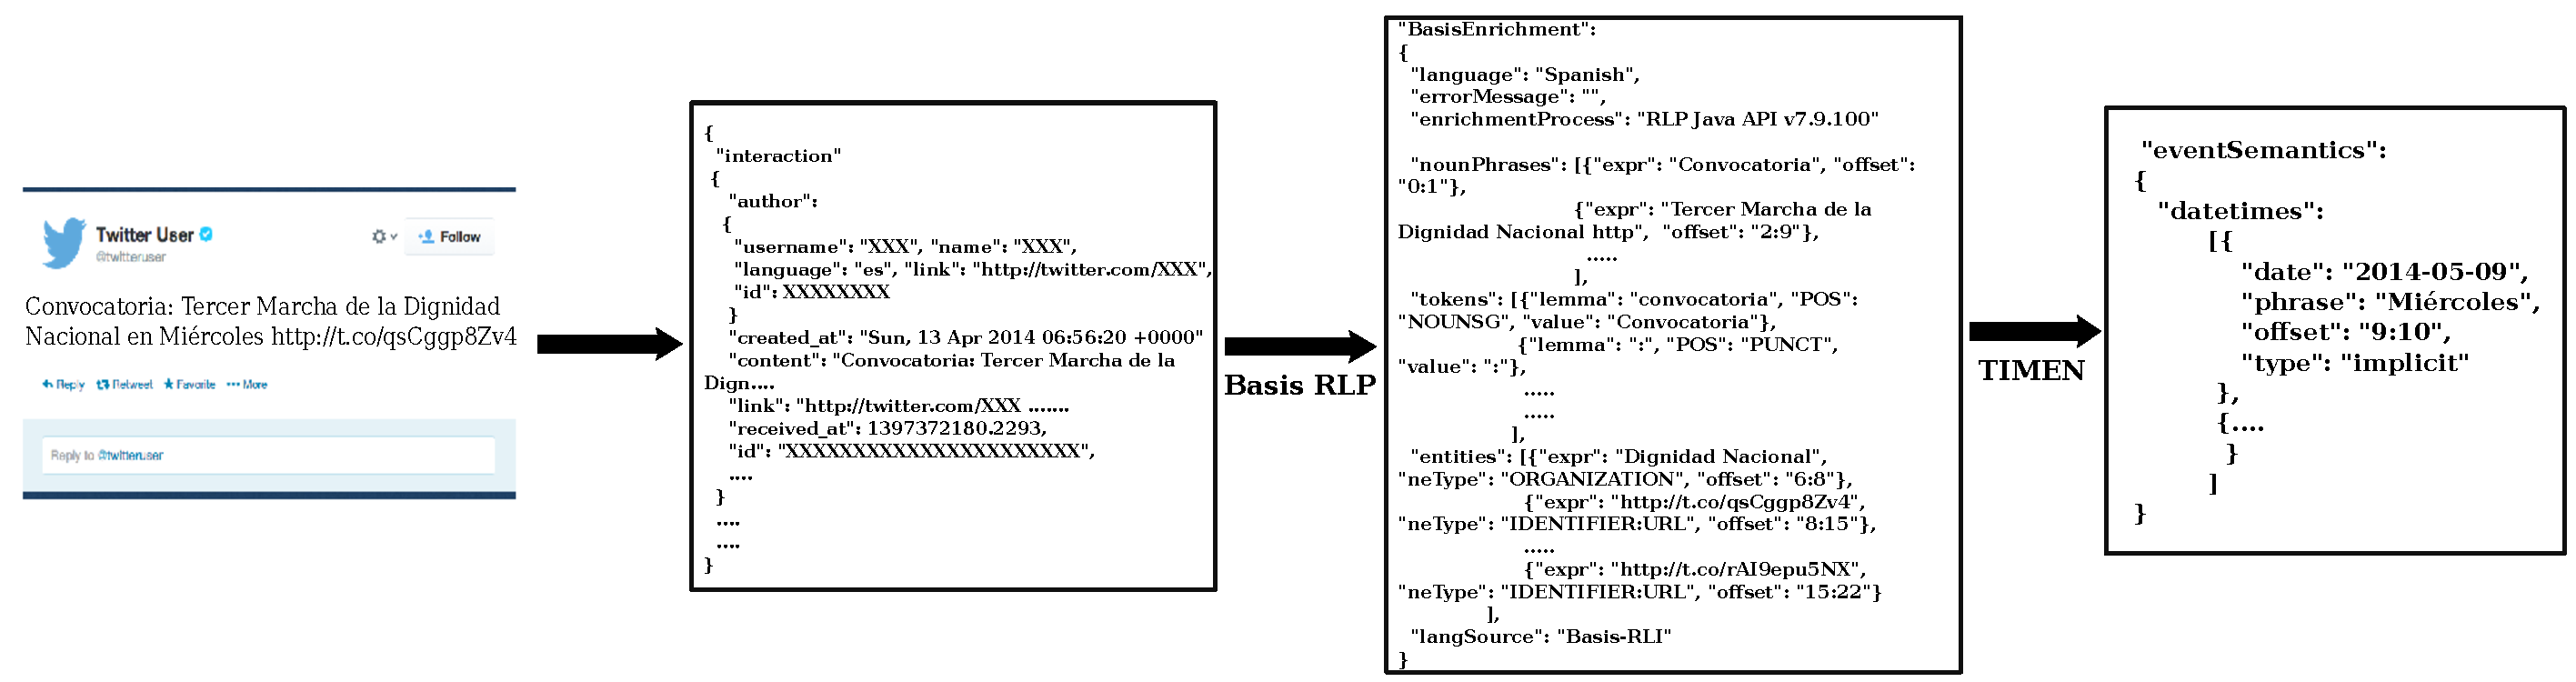
\includegraphics[width=0.5\textwidth]{enrichment}
    \caption{Message Enrichment}
    \label{fig:enrichment}
\end{figure}

Date processing is particularly crucial to the identification of
future oriented statements. We use the TIMEN \cite{LlorensDGS12} date
normalization package to normalize and deindex expressions referring
to days in English, Spanish and Portuguese.  This system makes use of
meta-data, such as the day of publication, and other information about
the linguistic context of the date expression to determine for each
date expression, what day (or week, month or year) it refers to.  For
example in a tweet produced on June 10, 2014, the occurrence of the
term {\em Friday} used in a future-tense sentence {\em We'll get
  together on Friday} will be interpreted as July 13, 2014.  Each
expression identified as a date by the RLP preprocessor is normalized
in this way.


\subsection{Geo-Coding}
\label{subsection:geocoding}

After linguistic preprocessing messages are geocoded with a
specification of the geographical focus of the text---specified as a
city, state, country tripple---that indicates the locality that the
text is ``about.'' We make use of different geocoding methodologies
for Twitter messages, for Facebook Events pages, and for news articles and blogs.
These are described below.


\subsubsection{Twitter}

For tweets, the geo-focus of the message is generated by a fairly
simple set of heuristics.  In particular, Twitter
geocoding is achieved by first considering the most reliable but least
available source, the geotag of the tweet itself (this is available
for about 10% of our sample from Twitter). This provide an exact
geographic locations that can be reverse geocoded into a place names
and this used as the geo-focus. We find the nearest geo-coded point in
our extended gazetteer (using the KD-Tree algorithm) for this
purpose. If the tweet is not geocoded, we consider Twitter ``places''
metadata and use place names present in these metadata fields to
geocode the place names into geographical coordinates.  Finally, if
none of this is available, we consider the text fields contained in
the user profile (location, description) as well as the tweet text
itself to find mentions of relevant locations.  Additional toponym disambiguiation heuristics are used to
identify the actual referent of the mention.

This simple set of heuristics achieves accuracy of ... 
(GRAHAM: RESULTS OF GEOCODING STUDY HERE)

\subsubsection{Facebook}
Similar methods are used to geocode event data extracted from Facebook Events pages.   Since only Facebook Events that have a venue are used and a venue of a Facebook Event generally contains a latitude, longitude, and physical address information identifying the locatino is a fairly trivial task.  In cases where only latitude and longitude are given we apply reverse-geocoding mechanisms similar to those used for Twitter.


\subsubsection{News/Blogs}

For longer articles such as news articles, the geo-focus of the message is identified using much more complex methods
To extract the protest location from news articles, we use \emph{probabilistic soft logic} (PSL) described in ~\ref{section:PSL} to build a model that performs robust, probabilistic inference given noisy signals. PSL takes a set of weighted, logic-like rules and converts them into a continuous probability distribution over the unknown truth values of logical facts. These truth values in PSL are relaxed into the $[0,1]$ interval. We use this mechanism to build a model that infers the semantic location of an article by weighing evidence coming from the Basis entity extractions and information in the World Gazatteer. 

The primary rules in the model encode the effect that Basis-extracted location strings that match to gazatteer aliases are indicators of the article's location, whether they be country, state, or city aliases. Each of these implications is conjuncted with an prior for ambiguous, overloaded aliases that is proportional to the population of the gazetteer location. For example, if the string ``Los Angeles'' appears in the article, it could refer to either Los Angeles, California, or Los \'{A}ngeles in Argentina or Chile. Given no other information, our model would infer a higher truth value for the article referring to Los Angeles, California, because it has a much higher population than the other options. 

\begin{flalign*}
    ENTITY&(L, location) \softand REFERSTO(L, locID) &\\
                        &\rightarrow PSLLOCATION(Article, locID) &
\end{flalign*}


\begin{flalign*}
    ENTITY&(C, location) \softand IsCountry(C) &\\
                        &\rightarrow ArticleCountry(Article, C) &
\end{flalign*}


\begin{flalign*}
    ENTITY&(S, location) \softand IsState(S)&\\
                            &\rightarrow ArticleCountry(Article, S)&
\end{flalign*}

The secondary rules, which are given half the weight of the primary rules, perform the same mapping of extracted strings to gazetteer aliases, but for extracted persons and organizations. Strings describing persons and organizations often include location clues (e.g., ``mayor of Buenos Aires''), but intuition suggests the correlation between the article's location and these clues may be lower than with location strings. 

\begin{flalign*}
    ENTITY&(O, organization) \softand REFERSTO(O, locID)&\\
                            &\rightarrow PSLLOCATION(Article, locID) &
\end{flalign*}


\begin{flalign*}
    ENTITY&(O, organization) \softand IsCountry(O)&\\
        &\rightarrow ArticleCountry(Article, O)&
\end{flalign*}


\begin{flalign*}
    ENTITY&(O, organization) \softand IsState(O)&\\
          &\rightarrow ArticleCountry(Article, O) &
\end{flalign*}
Finally, the model includes rules and constraints to require consistency between the different levels of geolocation, making the model place higher probability on states with its city contained in its state, which is contained in its country. As a post-processing step, we enforce this consistency explicitly by using the inferred city and its enclosing state and country, but adding these rules into the model makes the probabilistic inference prefer consistent predictions, enabling it to combine evidence at all levels.

\begin{flalign*}
    PSLLOCATION&(Article, locID) \softand Country(locID, C)&\\
               &\rightarrow ArticleCountry(Article, C)&
\end{flalign*}


\begin{flalign*}
    PSLLOCATION&(Article, locID) \softand Admin1(locID, S)&\\
               &\rightarrow ArticleState(Article, S)&
\end{flalign*}


\begin{figure*}
    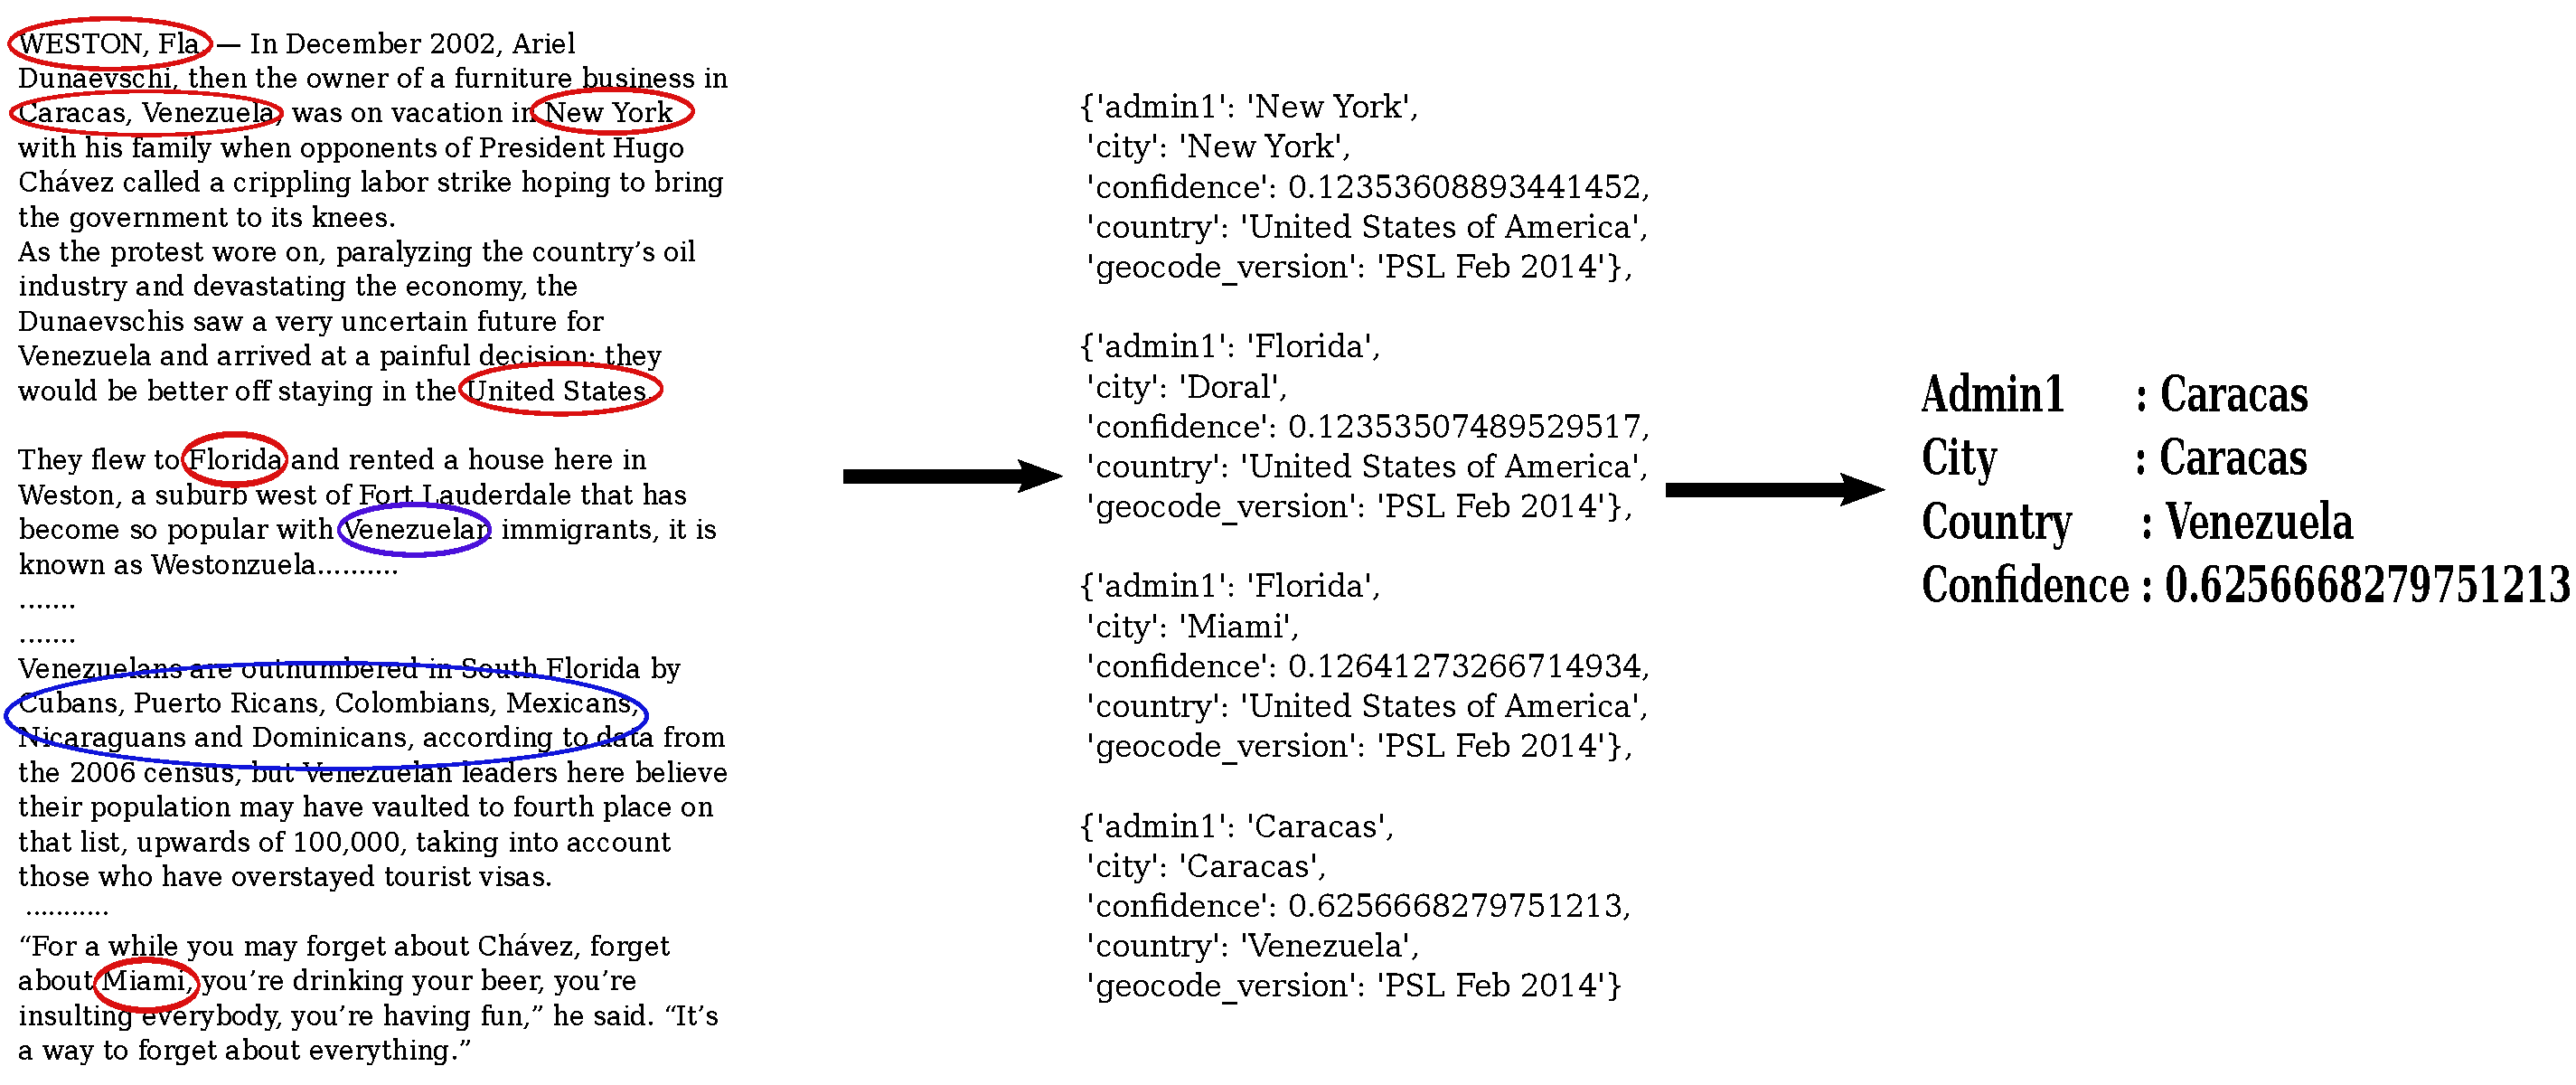
\includegraphics[width=\textwidth]{psl_pipeline}
    \caption{Red circles denote named entities identified as locations and blue denotes other types of entities. The article is reported from Weston Florida US and talks about the recent increase of venezuelan population in the US compared to other Latin American Nations like Cuba etc.\sathappanc{TODO: Replace with a better protest example}}
    \label{fig:psl_example}
\end{figure*}

(GRAHAM: DO WE WANT TO SUMMARIZE SOME RESULTS HERE TOO?)

%%!TEX root = ../plannedprotest.tex

To extract the protest location from news articles, we use \emph{probabilistic soft logic} (PSL) \cite{broecheler:uai10;kimmig:probprog12} to build a model that performs robust, probabilistic inference given noisy signals. PSL takes a set of weighted, logic-like rules and converts them into a continuous probability distribution over the unknown truth values of logical facts. These truth values in PSL are relaxed into the $[0,1]$ interval. We use this mechanism to build a model that infers the semantic location of an article by weighing evidence coming from the Basis entity extractions and information in the World Gazatteer. 

The primary rules in the model encode the effect that Basis-extracted location strings that match to gazatteer aliases are indicators of the article's location, whether they be country, state, or city aliases. Each of these implications is conjuncted with an prior for ambiguous, overloaded aliases that is proportional to the population of the gazetteer location. For example, if the string ``Los Angeles'' appears in the article, it could refer to either Los Angeles, California, or Los \'{A}ngeles in Argentina or Chile. Given no other information, our model would infer a higher truth value for the article referring to Los Angeles, California, because it has a much higher population than the other options. 

The secondary rules, which are given half the weight of the primary rules, perform the same mapping of extracted strings to gazetteer aliases, but for extracted persons and organizations. Strings describing persons and organizations often include location clues (e.g., ``mayor of Buenos Aires''), but intuition suggests the correlation between the article's location and these clues may be lower than with location strings. 

Finally, the model includes rules and constraints to require consistency between the different levels of geolocation, making the model place higher probability on states with its city contained in its state, which is contained in its country. As a post-processing step, we enforce this consistency explicitly by using the inferred city and its enclosing state and country, but adding these rules into the model makes the probabilistic inference prefer consistent predictions, enabling it to combine evidence at all levels.

\iffalse Most news articles and blog posts mention multiple locations, e.g.,
the location of reporting, the location of the incident, and locations corresponding
to the hometown of the newspaper. We developed a probabilistic reasoning
engine using probabilistic soft logic (PSL)
to infer the most likely city, state and country which is the main geographic focus the article.The PSL geocoder combines various types of evidence, such as named entities
such as locations, persons, and organizations identified by RLP, as
well as common names and aliases and populations of known
locations. These diverse types of evidence are used in weighted rules
that prioritize their influence on the PSL model's location
prediction. For example, extracted location tokens are strong
indicators of the content location of an article, while organization
and person names containing location names are weaker but still
informative signals; the rules corresponding to these evidence types
are weighted accordingly.

The methodology is similar to {\em Web-a-where: Geo-Tagging Web Content}.
\fi 

\begin{figure}
    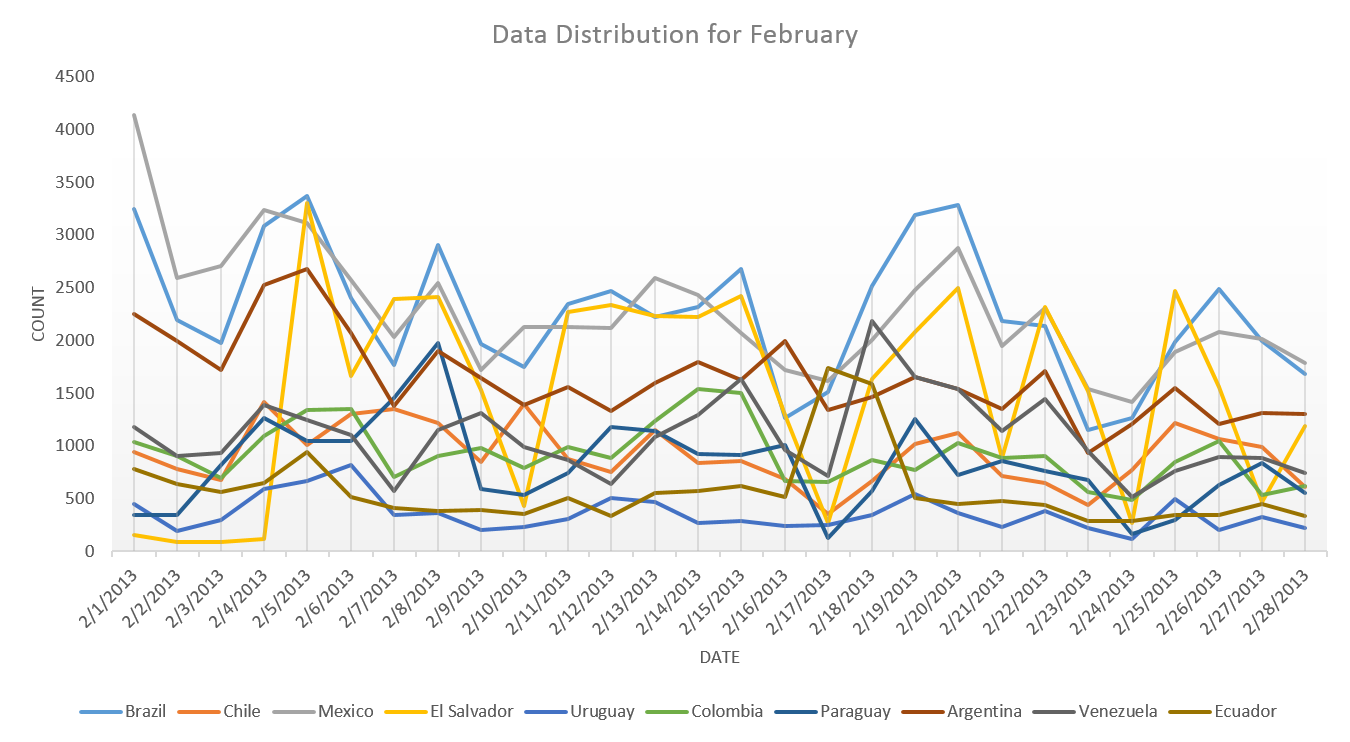
\includegraphics[width=0.5\textwidth]{rssdistribution}
    \caption{Rate of Arrival of News/Blogs}
    \label{fig:rssdistribution}
\end{figure}




\begin{figure*}
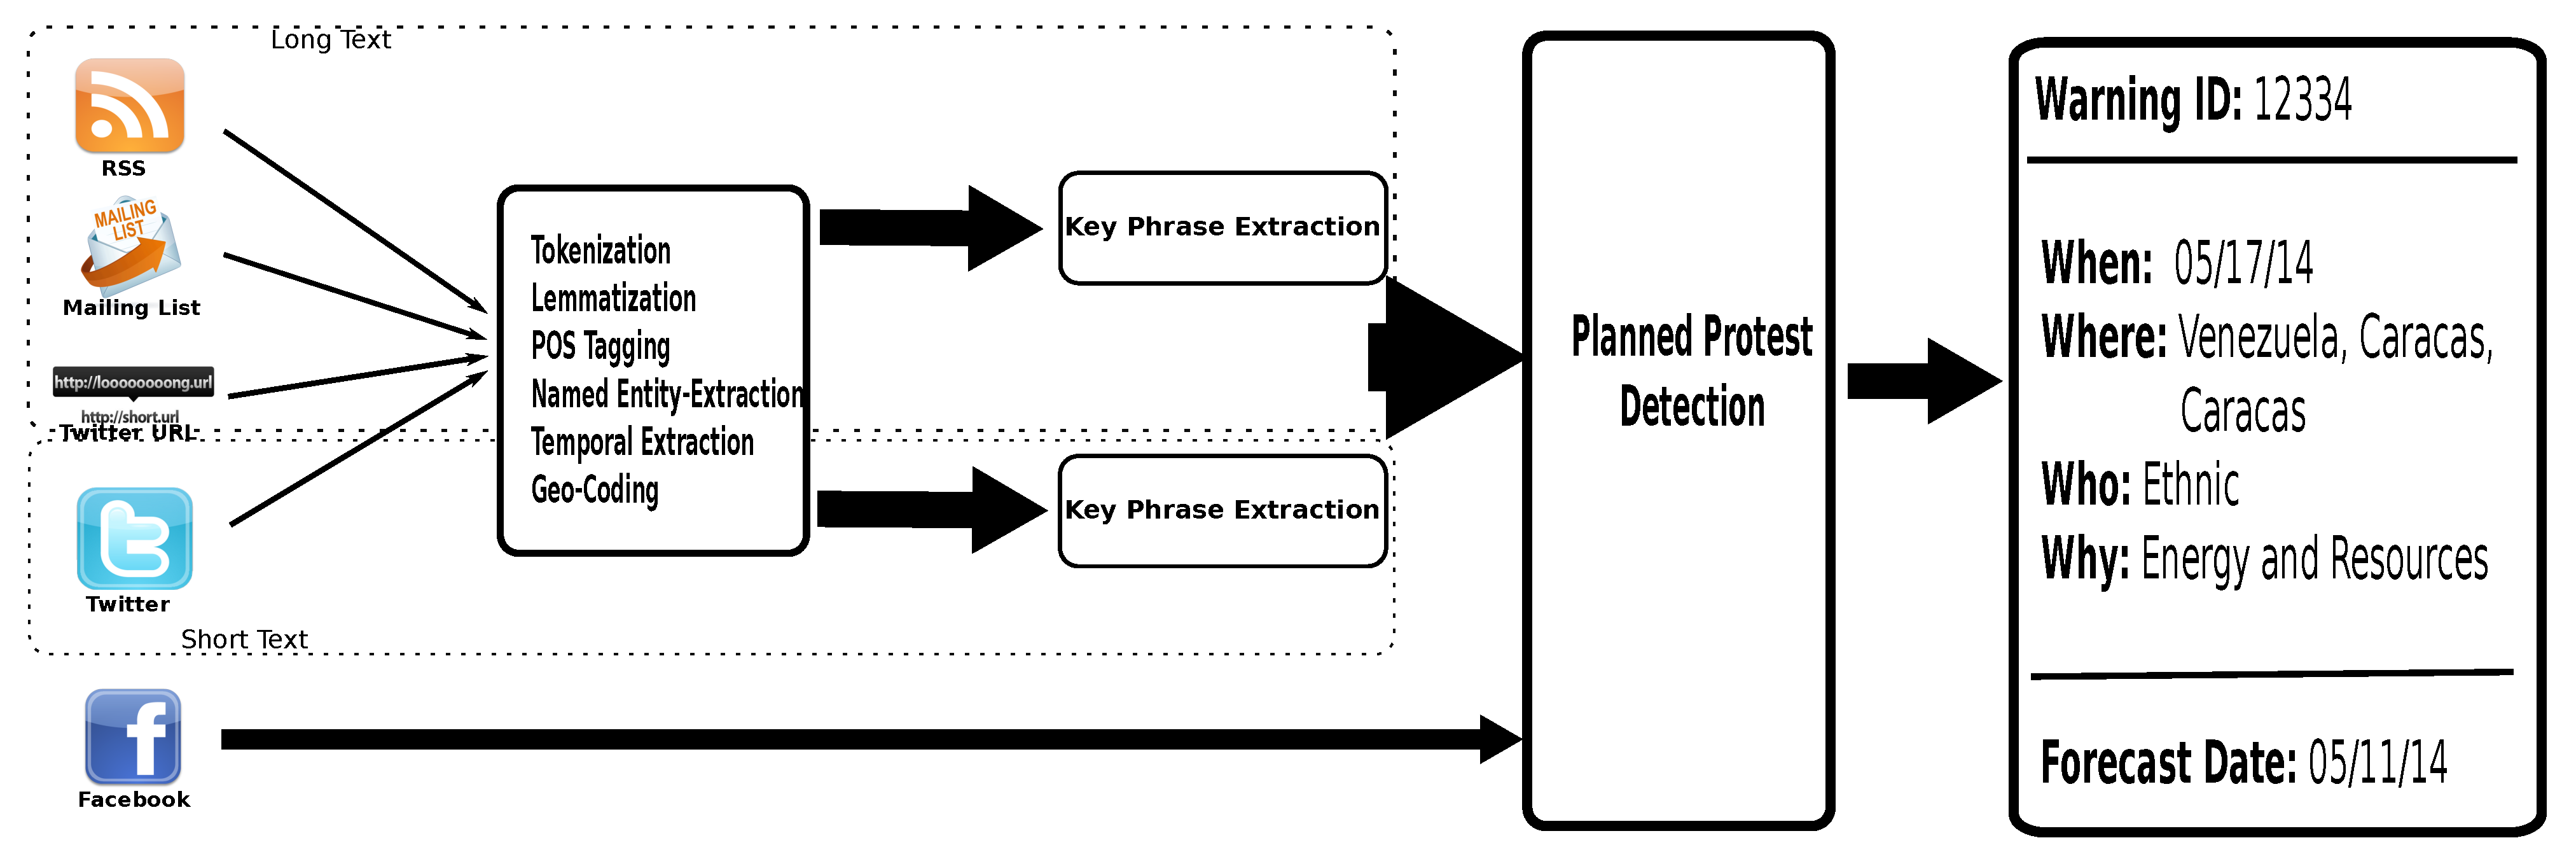
\includegraphics[width=\textwidth]{pp_pipeline}
\caption{A diagram showing various steps of the Model}
\end{figure*}

\subsection{Phrase filtering}

In order to identify relevant documents, input documents are filtered on a set of key phrases, that is 
the text of the document is searched for the presence of one or
more key phrases in a list of phrases which are indicative of an article's being
about a planned civil unrest event.  
The list of key phrases indicating civil unrest planning was obtained
in a semi-automatic manner, as detailed in Section \ref{sec:phraselearning}.
Articles which do match are processed further, those that do not are ignored.

\subsubsection{Phrase matching}

Our key phrase matching is highly general and linguistically
sophisticated.  The phrases in our list are general rules for
matching, rather than literal string sequences. Typically a phrase
specification consisting of two or more word lemmas, a language
specification and a separation threshold. This indicates that words -
potentially inflected forms - in a given sequence potentially
separated by one or more other words, should be taken to be a
``match.''   It was found that this kind of
multi-word key phrases was more accurate than simple keywords for
extracting events of interest from the data stream.

The presence of a keyphrase is checked by searching for the presence of
individual lemmas of the keyphrase within the same sentence separated
by at most a number of word that is fewer than the separation threshold.  
This method allows for linguistically sophisticated and flexible matching, so, for example,
they keyphrase [{\em plan protest}, 4, English] would match the sentence
{\em The students are planning a couple big protests tomorrow} in an input document.


\subsubsection{Phrase list development}
\label{sec:phraselearning}

The set of key phrases was tailored (slightly) the the genre of the
input. In particular different phrases were used to identify relevant
news articles and blogs from those used to filter Tweets.  The lists
themselves were generated semi-audomatically.

Initially, a few seed phrases were obtained manually
with the help of subject matter experts.
\sathappanc{Jaime's Text --> edited by graham}
An analysis of news reports for planned protests in the print media helped create a
minimum set of words to use in the query.  We choose four nouns from
the basic query that is used predominantly to indicate a civil unrest
in the print media - {\em demonstration, march, protest and
  strike}. We translated them into Spanish and Portuguese, including
synonyms.  We then combined these with future-oriented verbs - {\em to organize}, {\em to prepare}, {\em to
plan}, {\em to announce}, etc. For twitter, shorter phrases were identified, and these had
a more direct call for action, for example, {\em marchar}, {\em manhã de mobilização}, {\em
  vamos protestar}, {\em huelga}.

To generalize this set of phrases, the the phrases were then parsed
using a dependency parser \cite{freeling} and the grammatical
relationship between the core the nominal focus word (e.g., {\em
  protest}, {\em manifestación}, {\em huelga}) and any accompanying
word (e.g., {\em plan}, {\em call}, {\em anunciar}) was
extracted. These grammatical relations were used as extraction
patterns as in \cite{riloff2003learning} to learn more phrases from a
corpora of sentences extracted from the data stream of interest
(either news/blogs or tweets). This corpus consists of sentences that
contained any one of the nominal focus words and also had mentions of
a future date. The separation threshhold for a phrase was also
learned, being set is set to the average number of words separating
the nominal focus and the accompanying word.

The set of learned phrases is then reviewed by a subject matter expert for quality contraol.  
Using this approach, we learned 112 phrases for news articles and blogs and 156 for tweets.  
This phrase learning process is illustrated in Fig.~\ref{fig:phraselearning}



\begin{figure}
\caption{An Example of Phrase Learning}
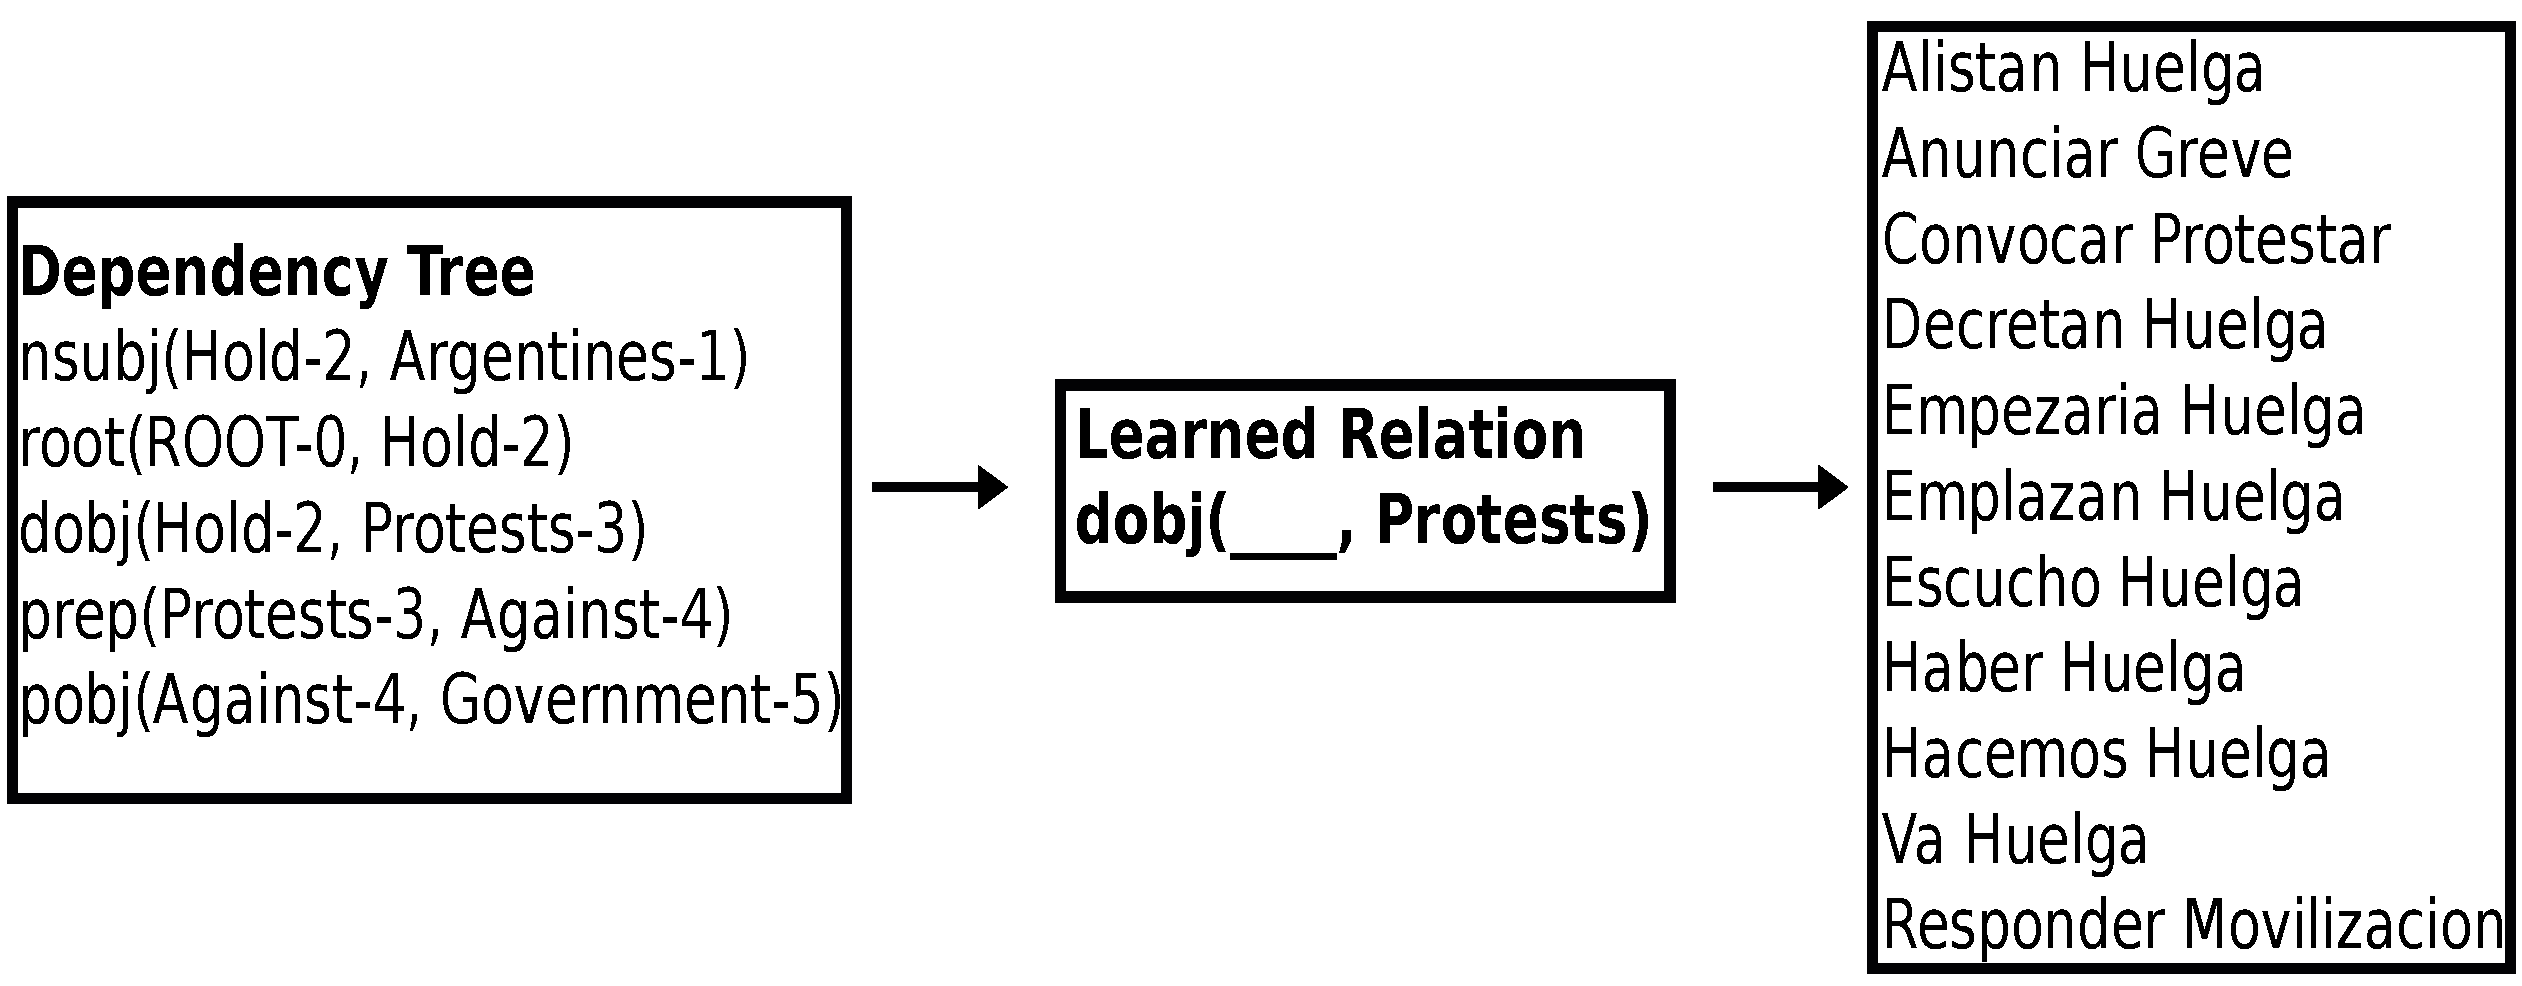
\includegraphics[width=0.5\textwidth]{figures/phraseLearning}
\label{fig:phraselearning}
\end{figure}

\subsection{Warning Generation}

After being subject to the preprocessing steps, above, all documents
that are identified as containing a key phrase are further filtered by
searching for the presence a future date in the passage containing the
key phrase and for the existence of an identified geographical focus for the text.
Documents that meet all these critera are used as the basis for a warning about a
planned civil unrest event (Twitter postings are only used as the basis for a warning
if the tweet is re-tweeted at least five times). 

A warning is generated for the date indicated by the future date
expression and the location which is the geographical focus of the
document.  For news articles and blog documents, information about
the event type and population for the event are derived from the
use of a text-based Naive Bayes classifier.  This classifier is
trained on the GSR and makes use of unigram and bi-gram word features.
For Twitter, since there is very little text in an individual tweet, the
event-type and population are based on based on prior likelihood for that location in the GSR.

In the case of Facebook, a Facebook-Event is considered to be good evidence for an alert if
there are more attendees for the event than rejects.  The date and
location are read off the Event page itself, and the population and event type are also based on priors.






\section{Experiments}
\begin{figure*}
\centering
\begin{subfigure}{\columnwidth}
  \centering
  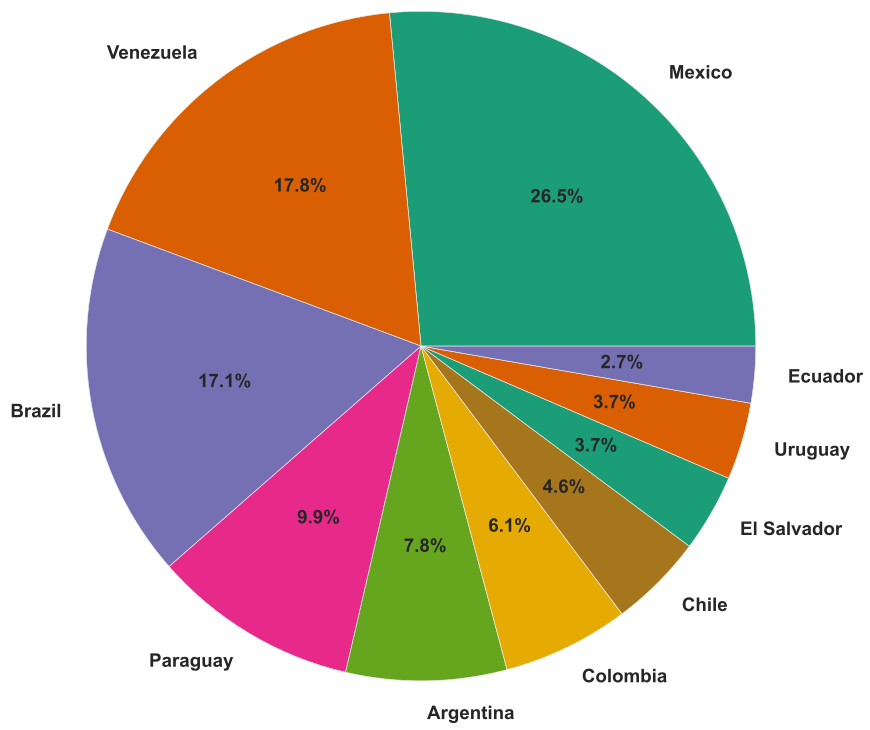
\includegraphics[scale=0.3]{gsr_distribution} 
  \caption{GSR distribution from 2012-11 to 2014-03.}
  \label{fig:gsrdistribution}
\end{subfigure}%
\begin{subfigure}{\columnwidth}
  \centering
  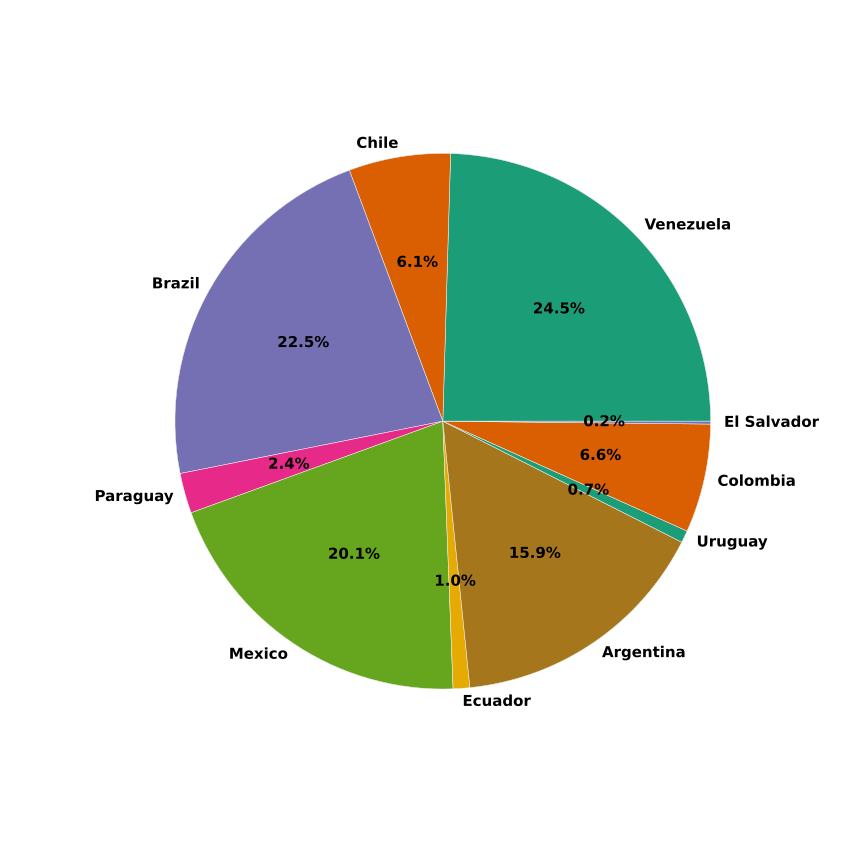
\includegraphics[scale=0.3]{pp_dist}
  \caption{Alerts distribution from 2012-11 to 2014-03.}
  \label{fig:ppdistribution}
\end{subfigure}
\caption{Distribution of alerts and GSR events across the Latin American countries studied in this paper.}
\label{fig:distribution}
\end{figure*}

We evaluate our planned protest detection system for Latin America using metrics similar to those described in 
~\cite{emberskdd}.
Given a set of alerts issued by the system and the GSR comprising actual protest incidents, we aim to identify
a correspondence between the two sets via a bipartite matching.
An alert can be matched to a GSR event only if i) they are both issued for the same country, 
ii) the alert's predicted location and the event's reported location are within 300km of each
other (the distance offset), and iii) the forecast event date is within a given interval of the true event date (the date offset).
Once these inclusion criteria apply, the quality score (QS) of the match is defined as a combination of the
location score (LS) and date score (DS):
\small
\begin{equation}
    \operatorname{QS}= (LS + DS)*2
\end{equation}
\normalsize
\noindent
where
\small
\begin{equation}
    \operatorname{LS}=1 - \frac{\min(\textrm{distance offset}, 300)}{300}
\end{equation}
and 
\begin{equation}
    \operatorname{DS}=1 - \frac{\min(\textrm{date offset}, \operatorname{INTERVAL})}{\operatorname{INTERVAL}}
\end{equation}
\normalsize
Here, we explore $\operatorname{INTERVAL}$ values from $0$ to $7$.
if an alert (conversely, GSR event) cannot be matched to any GSR event (alert, respectively), these unmatched
alerts (and events) will negatively impact the precision (and recall) of the system. The lead time,
for a matched alert-event pair,
is calculated as the difference between the date on which the forecast was made and the date on which the event
was reported (this should not be confused with the date score, which is the difference between the
predicted event date and the actual event date). Lead time concerns itself with reporting and forecasting, whereas
the date score is concerned with quality or accuracy.

We conduct a series of experiments to evaluate the performance of our system.\\

\noindent
{\bf How does the distribution of protests detected by the system compare with the
actual distribution of protests in the GSR?}
Fig.~\ref{fig:distribution} reveals pie charts of both distributions. As shown, Mexico, Brazil, and Venezuela
experience the lion's share of protests in our region of interest, and the protests detected also match these modes
although not the specific percentages. The smaller countries like Ecuador, El Salvador, and Uruguay do experience
protests but which are not as prominently detected as those for other countries; we attribute this to their smaller
social media footprint (relative to countries like Brazil and Venezuela).\\

\begin{table*}
    \centering
    \caption{\label{tb:sourcewisecomparison} 
    Country-wise breakdown of forecasting performance for different data sources.
QS=Quality Score; Pr=Precision; Rec=Recall; LT=Lead Time.
AR=Argentina; BR=Brazil; CL=Chile; CO=Colombia; EC=Ecuador;SV=El Salvador; 
MX=Mexico; PY=Paraguay; UY=Uruguay; VE=Venezuela. A $-$
indicates that the source did not produce any warnings for that country
in the studied period.}
\begin{tabular}{*{17}{|c}|}
        \toprule
        & \multicolumn{4}{ |c| }{News/Blogs} & \multicolumn{4}{ |c| }{Twitter} & \multicolumn{4}{ |c| }{Facebook} & \multicolumn{4}{ |c| }{Combined}\\
        \midrule
         & QS & Pr. & Rec. &LT & QS & Pr. & Rec. & LT & QS & Pr. & Rec. & LT & QS & Pr. & Rec. & LT\\
        \midrule
        AR &3.14&0.32&0.69&3.94&3.52&{\bf0.78}&0.14&3.14&{\bf3.70}&0.50&0.04&3.00&3.02&0.36&{\bf0.80}&{\bf4.50}\\
        BR &3.14&0.48&0.54&{\bf5.85}&-&-&-&-&{\bf3.62}&{\bf0.76}&0.18&2.46&3.28&0.49&{\bf0.65}&5.15\\
        CL &3.06&0.91&0.67&5.40&{\bf3.52}&{\bf1.00}&0.23&4.29&-&-&-&-&3.16&0.83&{\bf0.80}&{\bf5.92}\\
        CO &2.74&0.90&0.56&{\bf7.44}&3.30&{\bf1.00}&0.15&2.43&{\bf4.00}&{\bf1.00}&0.02&2.00&2.88&0.84&{\bf0.65}&6.47\\
        EC &-&-&-&-&{\bf2.32}&{\bf1.00}&{\bf0.06}&{\bf17.00}&-&-&-&-&{\bf2.32}&{\bf0.50}&{\bf0.06}&{\bf17.00}\\
        MX &2.96&0.88&0.25&{\bf3.69}&3.14&{\bf1.00}&0.02&1.43&{\bf3.72}&0.67&0.01&2.00&3.00&0.87&{\bf0.27}&3.51\\
        SV &{\bf3.22}&{\bf1.00}&{\bf0.03}&{\bf1.0}&-&-&-&-&-&-&-&-&{\bf3.22}&{\bf1.0}&{\bf0.03}&{\bf1.0}\\
        PY &3.38&{\bf1.00}&{\bf0.16}&9.11&3.84&{\bf1.00}&0.04&{\bf11.40}&3.96&{\bf1.00}&0.01&2.00&3.60&0.96&{\bf0.20}&9.35\\
        UY &{\bf3.24}&{\bf1.00}&{\bf0.29}&{\bf2.40}&-&-&-&-&-&-&-&-&3.24&{\bf1.00}&{\bf0.29}&3.24\\
        VE &{\bf3.80}&{\bf1.00}&0.36&{\bf3.27}&3.68&0.97&0.33&2.39&-&-&-&-&3.64&0.99&{\bf0.69}&2.88\\
        ALL &3.34&0.69&0.35&{\bf4.57}&3.62&{\bf0.97}&0.15&2.82&3.66&0.74&0.03&2.44&3.36&0.73&{\bf0.51}&4.08\\
        \bottomrule
    \end{tabular}
\end{table*}
\noindent
{\bf Are there country-specific selective superiorities for the different data sources considered here?}
Table~\ref{tb:sourcewisecomparison} presents a breakdown of perfomance, country-wise and source-wise, of 
our approach for a recent month, viz. March 2014.
It is clear that the multiple data sources are necessary to achieve a high recall and that by and large
these sources are providing mutually exclusive alerts. (Note also that some data sources do not produce alerts for specific
countries.) Between Twitter and Facebook, the former is a better
source of alerts for countries like Chile and the latter is a better source for Argentina, Brazil, Colombia, and Mexico.
News and blogs achieve higher recall than social media sources indicating that most plans for protests are announced
in established media. They are also
higher quality sources for alerts in countries like El Salvador, Paraguay, and Uruguay.
Finally, note that news and blogs offer a much higher lead time (4.57 days) 
as compared to that for Facebook (2.44 days) or for Twitter (2.82 days). The quality scores are
further broken down in Table~\ref{tb:modelwisecomparison} into their date and location components.

\begin{figure}[!ht]
    \vspace{-1em}
    \centering
    
\includegraphics[scale=0.3]{monthlyqs}
    \vspace{-.5em}
    \caption{Quality Score over the months}
    \label{fig:monthlyqs}
    \vspace{-1.5em}
\end{figure}
A longitudunal perspective on quality scores is
given in Fig.~\ref{fig:monthlyqs}. Note that in general Twitter tends to have a higher quality score
as multiple re-tweets of future event mentions is a direct indicator of the popularity of an event as 
well as the intent of people to join an event. 
In contrast, mentions of future events in news do not directly shed any insight into popularity or people's
support for the event's causes.\\

\begin{table*} %[tb!]
\centering
\caption{Comparing the location and date scores of different sources in specific countries.
AR=Argentina; BR=Brazil; CL=Chile; CO=Colombia; EC=Ecuador;SV=El Salvador; MX=Mexico; PY=Paraguay; UY=Uruguay; VE=Venezuela. A $-$ indicates that the source did not produce any warnings for that country in the studied period.}
\label{tb:modelwisecomparison}
\begin{tabular}{|l|*{17}{c|}}
\toprule
Source& & AR & BR & CL & CO & EC & SV & MX & PY & UY & VE & All\\
\toprule
\multirow{2}{*}{News/Blogs} &LS &0.82&0.76&0.75&0.60&-&{\bf0.75}&0.66&0.79&{\bf0.79}&{\bf0.95}&0.81\\
                            &DS&0.75&0.81&0.78&0.77&-&{\bf0.86}&0.82&0.90&{\bf0.83}&{\bf0.95}&0.86\\
\midrule
\multirow{2}{*}{Facebook} &LS &{\bf1.0}&{\bf0.92}&-&{\bf1.00}&-&-&{\bf0.86}&{\bf0.98}&-&-&{\bf0.93}\\
                          &DS&0.85&{\bf0.89}&-&{\bf1.00}&-&-&{\bf1.00}&{\bf1.00}&-&-&0.90\\
\midrule
\multirow{2}{*}{Twitter} &LS &0.88&-&{\bf0.84}&0.81&{\bf0.45}&-&0.71&{\bf0.98}&-&0.91&0.89\\
                         &DS&{\bf0.88}&-&{\bf0.92}&0.84&{\bf0.71}&-&0.86&0.94&-&0.93&{\bf0.92}\\
\bottomrule
\end{tabular}
\end{table*}

\noindent
{\bf How did our system fare in detecting key country-wide protests?}
\begin{figure*}
  \begin{subfigure}{\columnwidth}
    \centering
    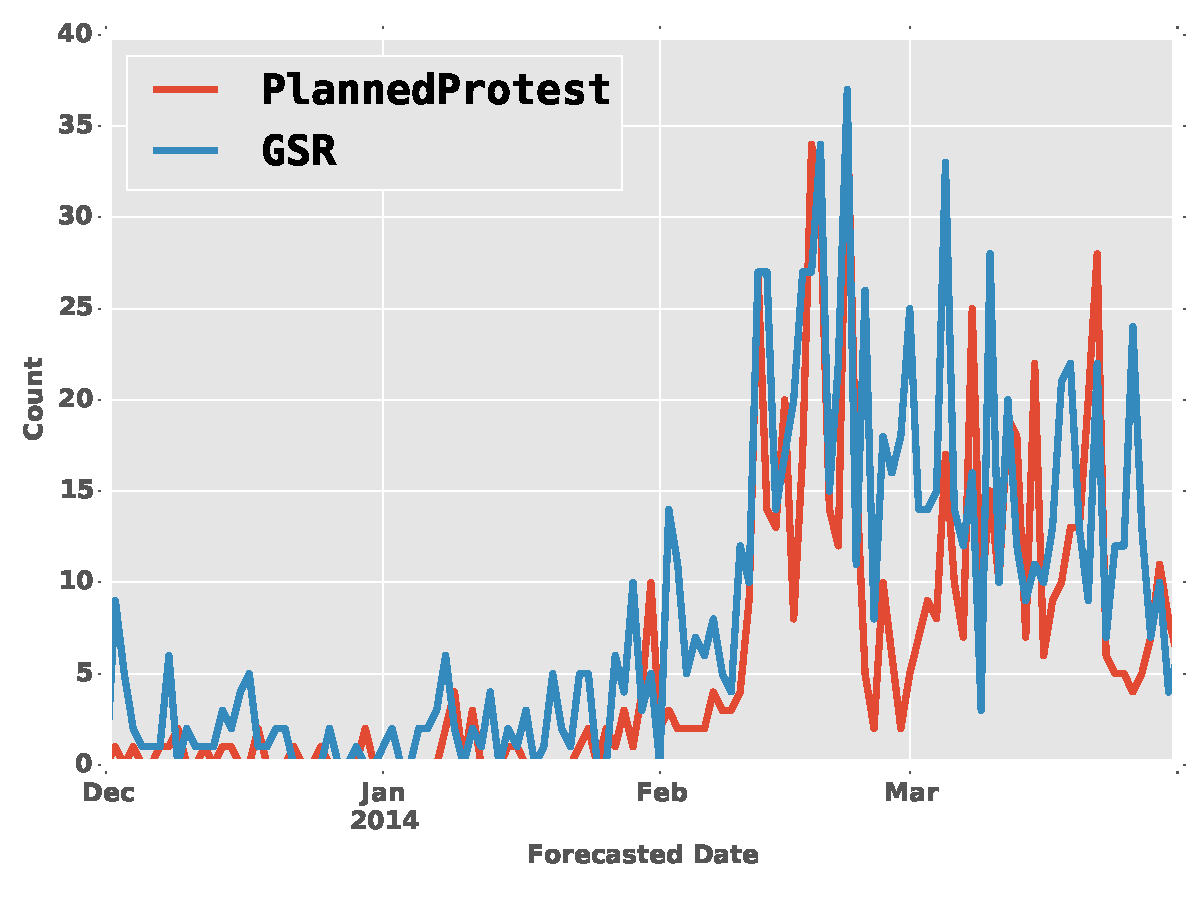
\includegraphics[scale=0.3]{venezuela_new}
    \caption{Venezuelan protests}
    \label{fig:venezuela_feb}
\end{subfigure}
\begin{subfigure}{\columnwidth}
    \centering
    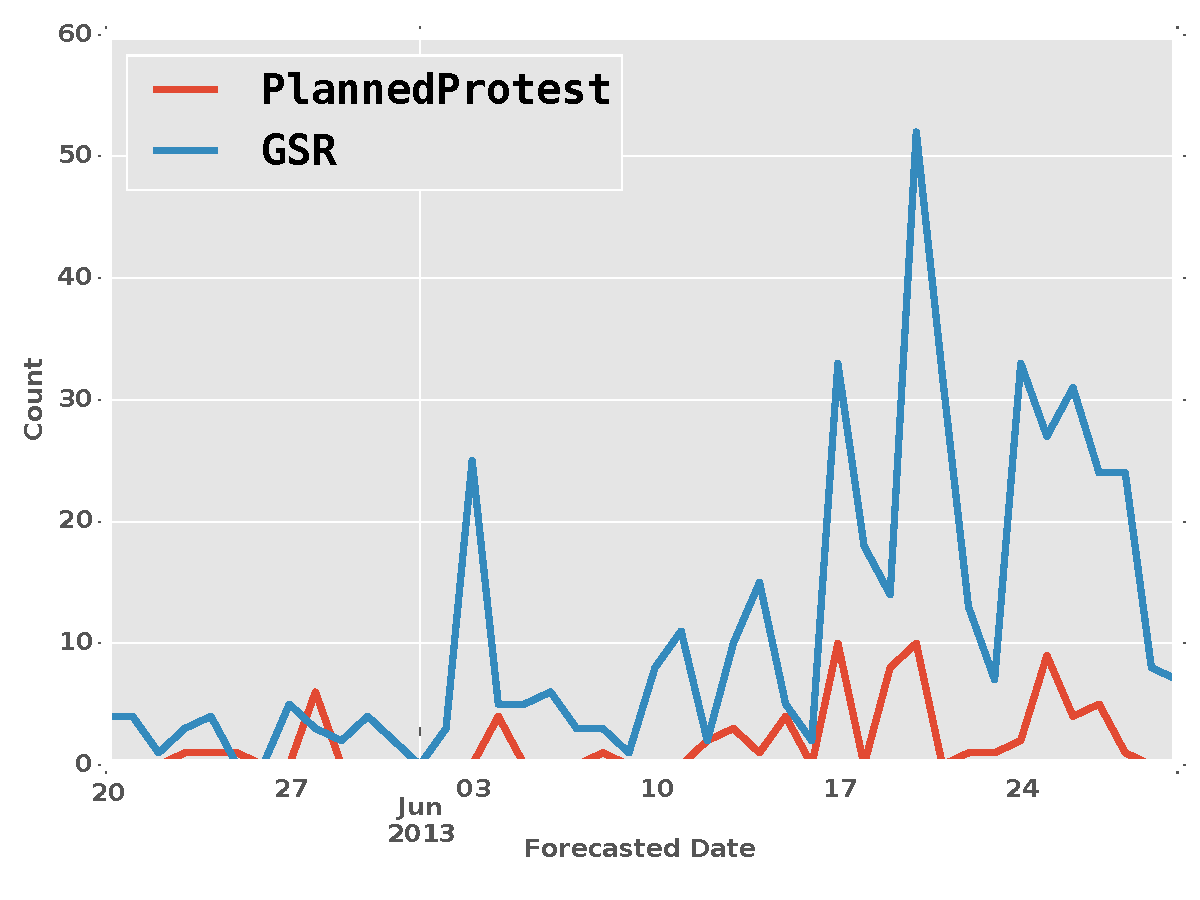
\includegraphics[scale=0.3]{brazil_june_new}
    \caption{Brazilian Spring}
    \label{fig:brazil_june}
\end{subfigure}
\caption{Mass protests forecast by our system}
\end{figure*}

The recent Venezuelan protests against President Nicolas Maduro and the Brazilian protests during June 2013 against bus fare hike were two significant protests during our period of evaluation. Fig.~\ref{fig:venezuela_feb} and
Fig.~\ref{fig:brazil_june} describe our performance under these two situations illustrating the count
of protests detected against the GSR. Notice that our system was able to 
identify the Venezuelan protests much better than the Brazilian protests. This is because there was a significant amount
of spontaineity to the Brazilian protests; they arose as discontent about bus fare increases but later morphed into a broader
set of protests against government and most of these subsequent protests were not planned.\\

\noindent
{\bf What is the tradeoff between lead time and quality?}

\begin{figure}[h!]
    \vspace{-1em}
    \centering
    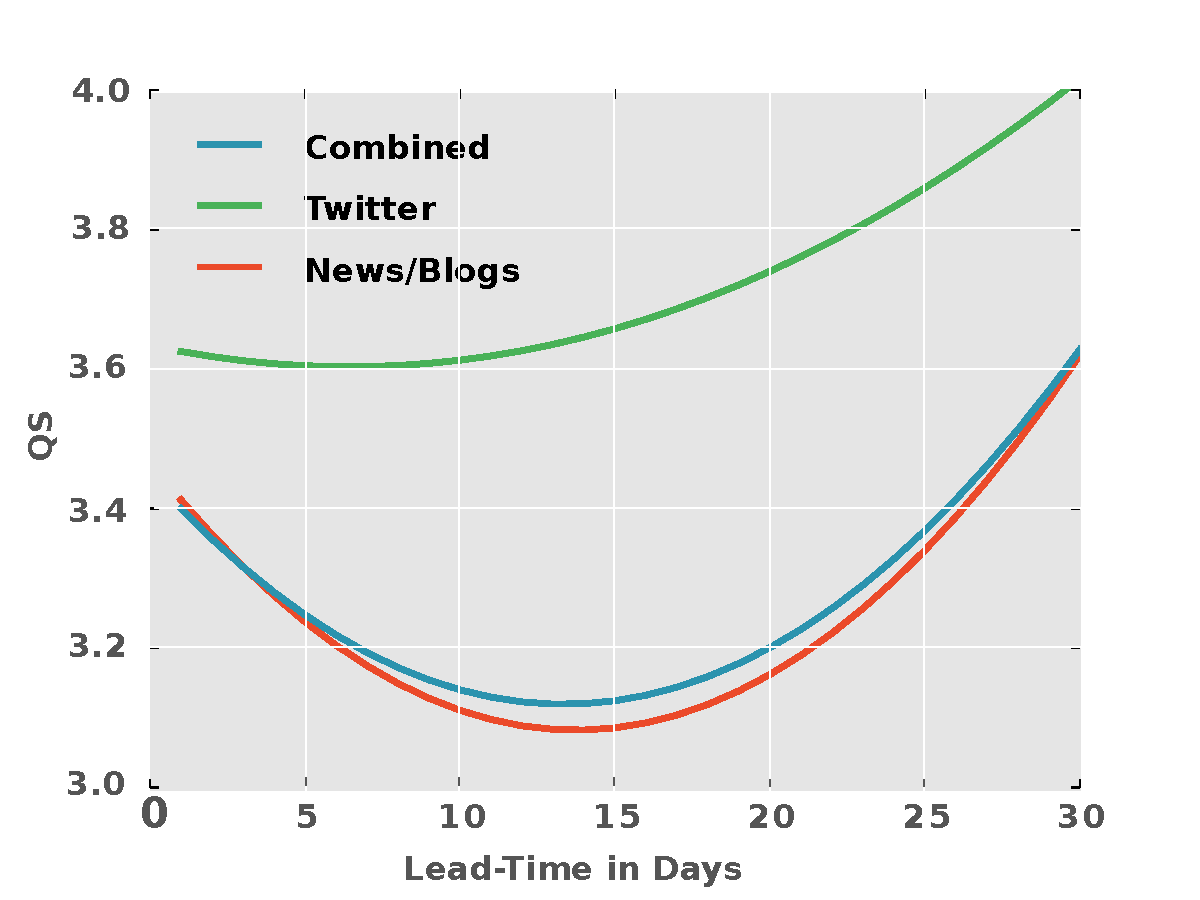
\includegraphics[scale=0.3]{leadTimeVsQS}
    \caption{Lead-Time vs Quality Score}
    \label{fig:leadTimeVsQS}
    \vspace{-1em}
\end{figure}

Fig.~\ref{fig:leadTimeVsQS} shows that the QS of the planned protest model decreases (as expected) with lead time, initially, but
later rises again. The higher quality scores toward the right of Fig.~\ref{fig:leadTimeVsQS} are primarily due to
Facebook event pages.\\

\noindent
{\bf How does the method perform under stringent matching criteria?}
Fig.~\ref{fig:matchinginterval} shows the perfomance of the model when the matching window is varied from 7 to 1 in steps. 
We can see that the performance degrades quite gracefully even under the strict matching interval of a 1-day difference.\\
\begin{figure}[h!]
    \vspace{-1em}
    \centering
  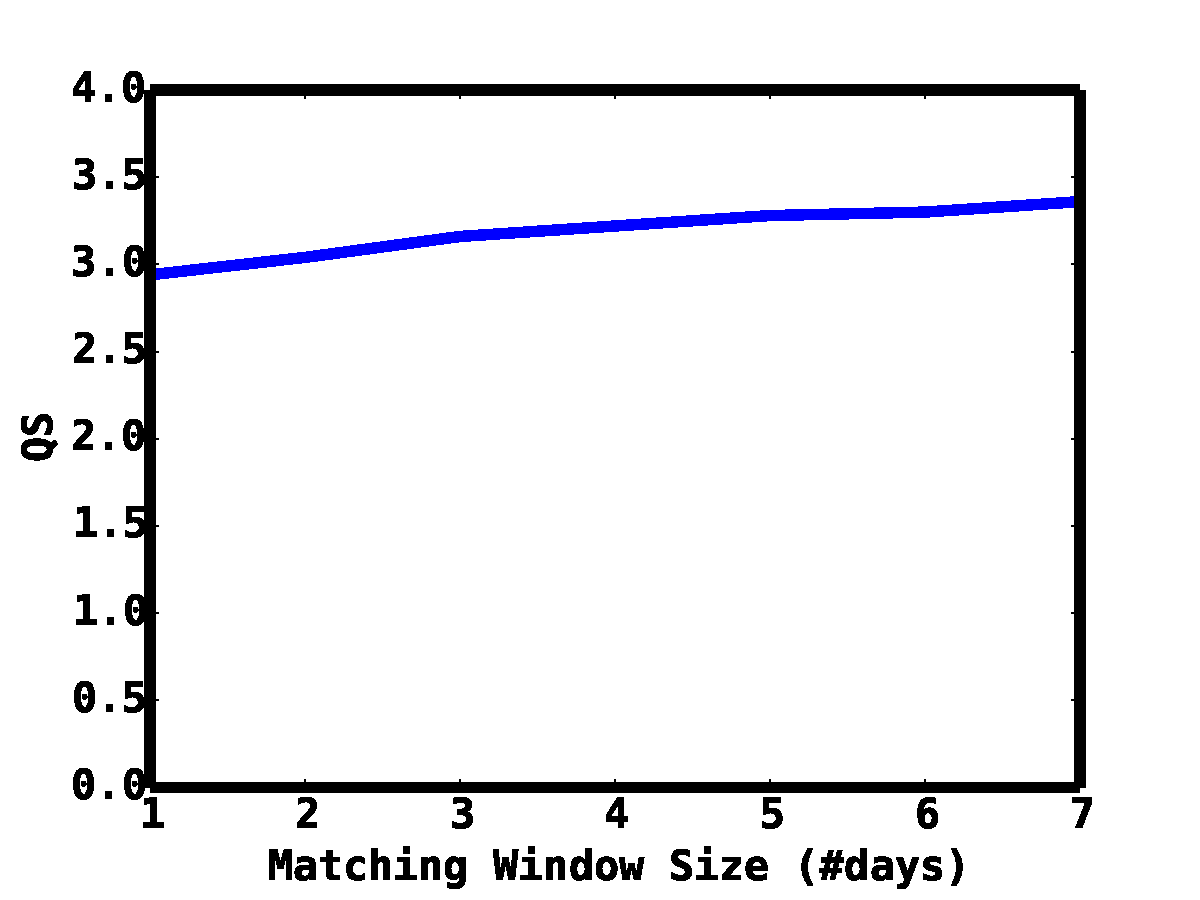
\includegraphics[scale=0.3]{matchingwindow}
    \vspace{-.5em}
  \caption{QS vs Matching Interval Trade-Off}
  \label{fig:matchinginterval}
    \vspace{-1.5em}
\end{figure}

\noindent
{\bf What is the distribution of quality scores?}
The clear mode toward the right side of the Fig.~\ref{fig:doubleHump} signifies that a majority of the planned 
protest alerts are of high quality. Further, the quality score distribution is unimodal suggesting that the careful reasoning of locations and date normalization are crucial to achieving high quality.
\begin{figure}[h!]
    \centering
  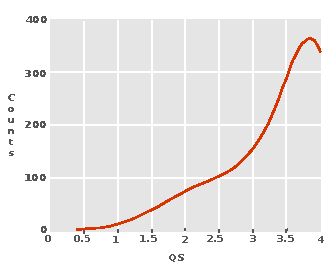
\includegraphics[scale=1]{doubleHump_new3}
    \vspace{-.5em}
  \caption{Quality Score Distribution}
  \label{fig:doubleHump}
    \vspace{-1.5em}
\end{figure}
%\begin{figure*}
%\begin{subfigure}{.70\columnwidth}
%    \centering
%  
\includegraphics[scale=0.2]{monthlyqs}
%  \caption{\scriptsize Quality Score over the months}
%  \label{fig:monthlyqs}
%\end{subfigure}\hspace{.5pt}
%\begin{subfigure}{.70\columnwidth}
%    \centering
%  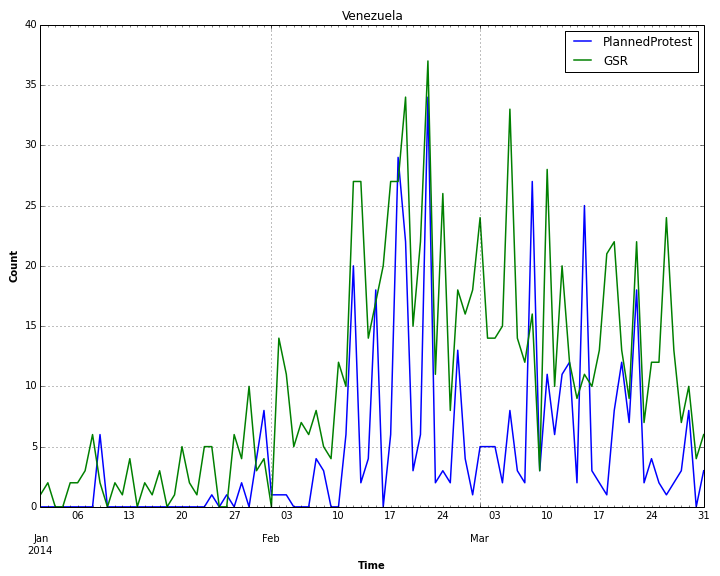
\includegraphics[scale=0.2]{venezuela}
%  \caption{\scriptsize Venezuelan Protests}
%  \label{fig:venezuela_feb}
%\end{subfigure}\hspace{.5pt}
%\begin{subfigure}{.70\columnwidth}
%    \centering
%  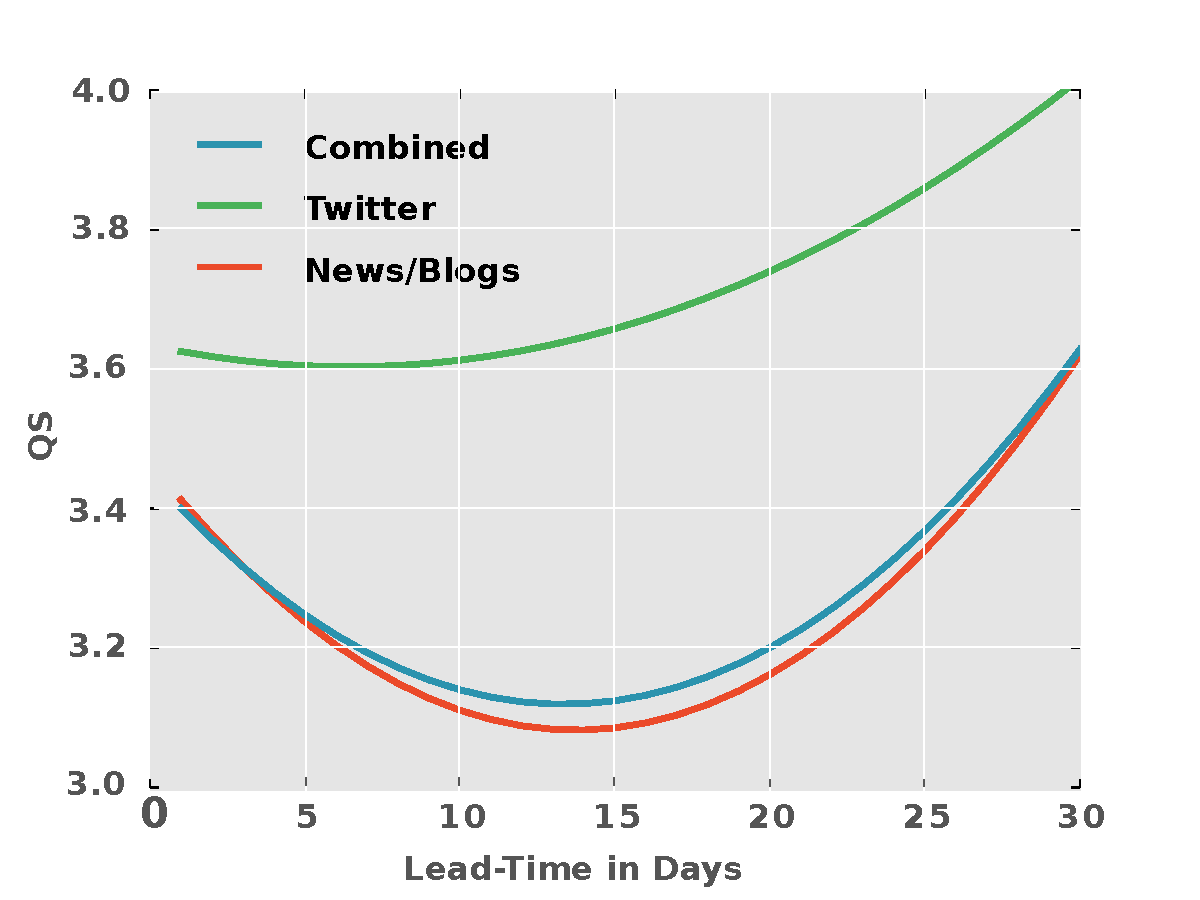
\includegraphics[scale=0.2]{leadTimeVsQS}
%  \caption{\scriptsize Lead-Time vs Quality Score}
%  \label{fig:leadTimeVsQS}
%\end{subfigure}
%
%\begin{subfigure}{.70\columnwidth}
%    \centering
%  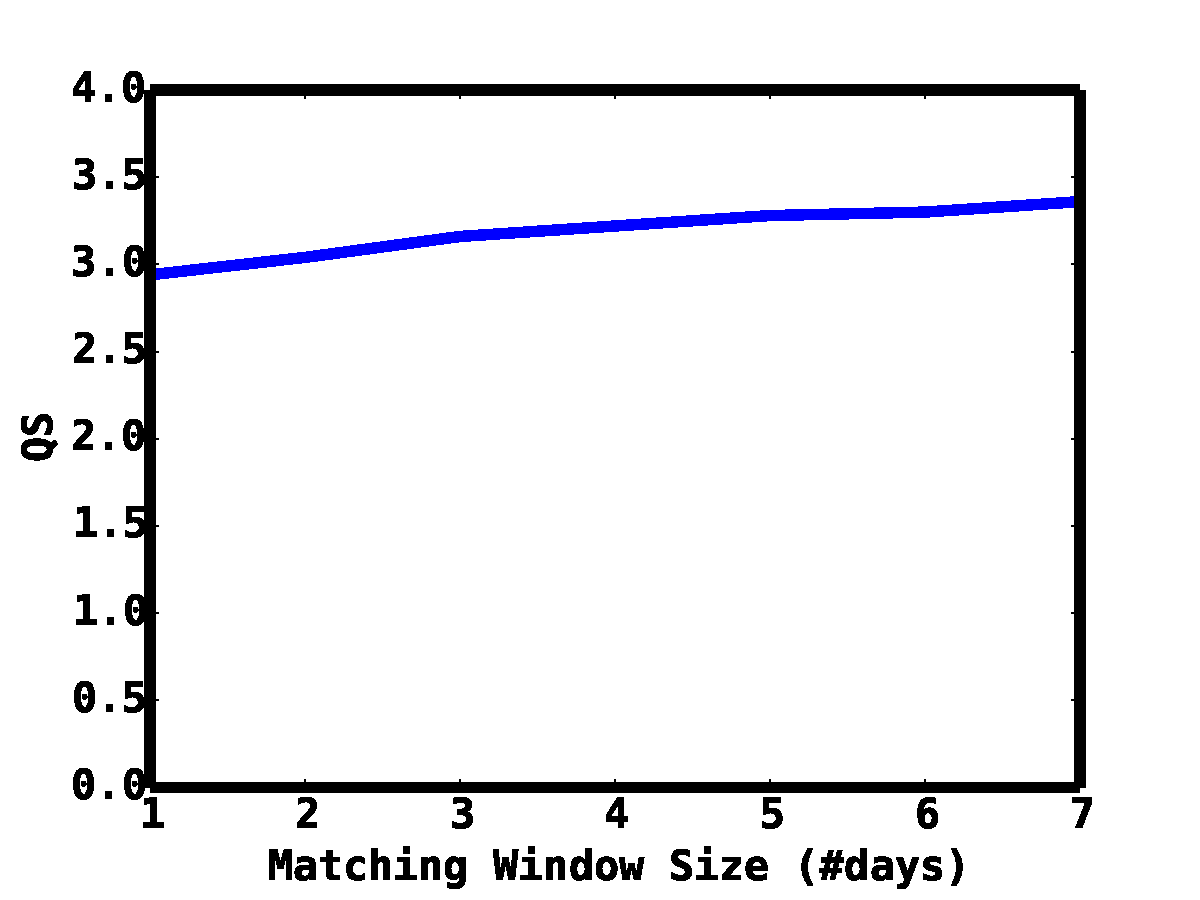
\includegraphics[scale=0.2]{matchingwindow}
%  \caption{\scriptsize QS vs Matching Interval Trade-Off}
%  \label{fig:matchinginterval}
%\end{subfigure}\hspace{.5pt}
%\begin{subfigure}{.70\columnwidth}
%    \centering
%  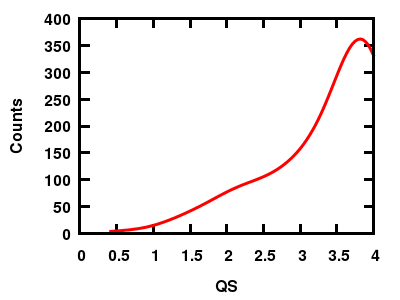
\includegraphics[scale=0.33]{doubleHump}
%  \caption{\scriptsize Quality Score Distribution}
%  \label{fig:doubleHump}
%\end{subfigure}\hspace{.5pt}
%\begin{subfigure}{.70\columnwidth}
%    \centering
%  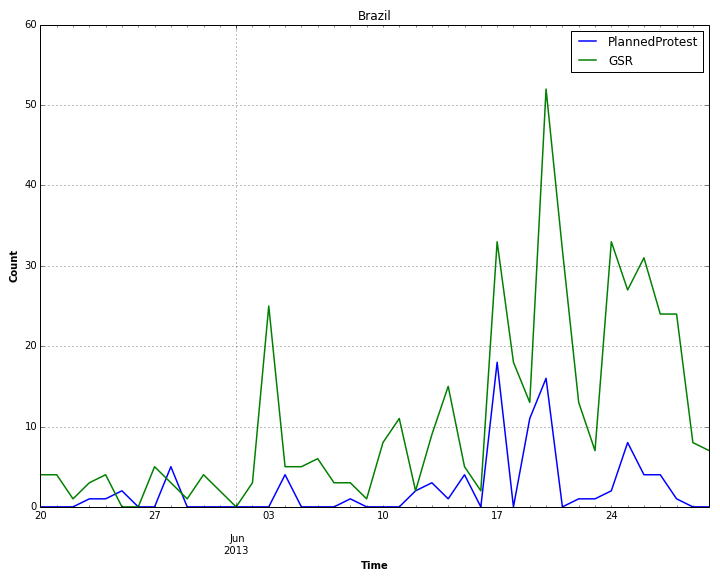
\includegraphics[scale=0.2]{brazil_june}
%  \caption{\scriptsize System Performance during Brazilian Spring}
%  \label{fig:brazil_june}
%\end{subfigure}\hspace{.5pt}
%\caption{Evaluation of planned protest forecasting system}
%\end{figure*}

%\begin{subfigure}{\columnwidth}
%  \centering
%  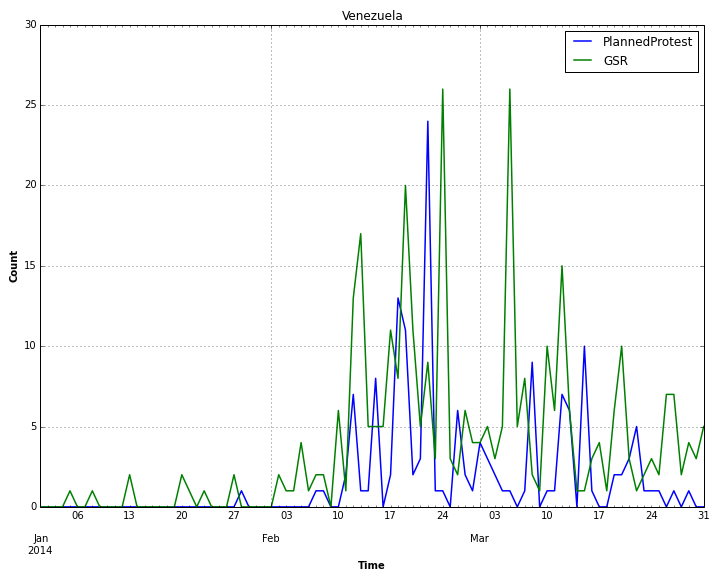
\includegraphics[width=\linewidth]{venezuela_violent}
%  \caption{Venezuelan Violent Protests}
%  \label{fig:venezuela_violent}
%\end{subfigure}%


%\begin{figure}
%    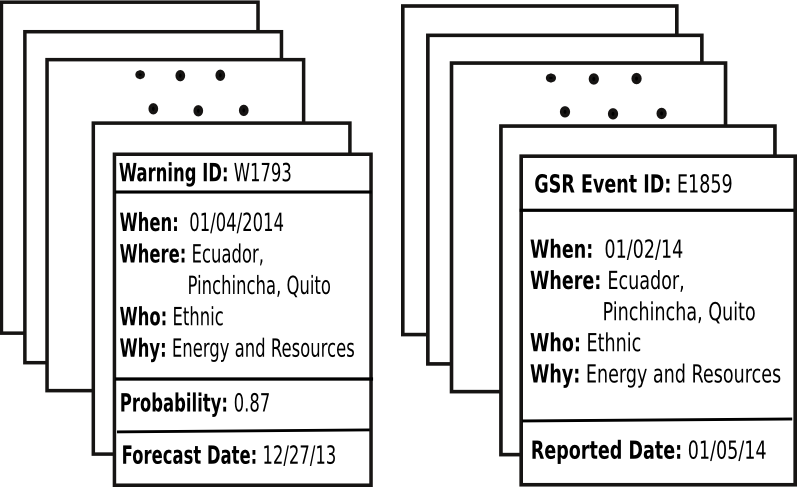
\includegraphics[width=0.5\textwidth]{alertstructure}
%    \caption{Structure of an Alert}
%    \label{fig:alertstructure}
%\end{figure}
%\begin{figure}
%    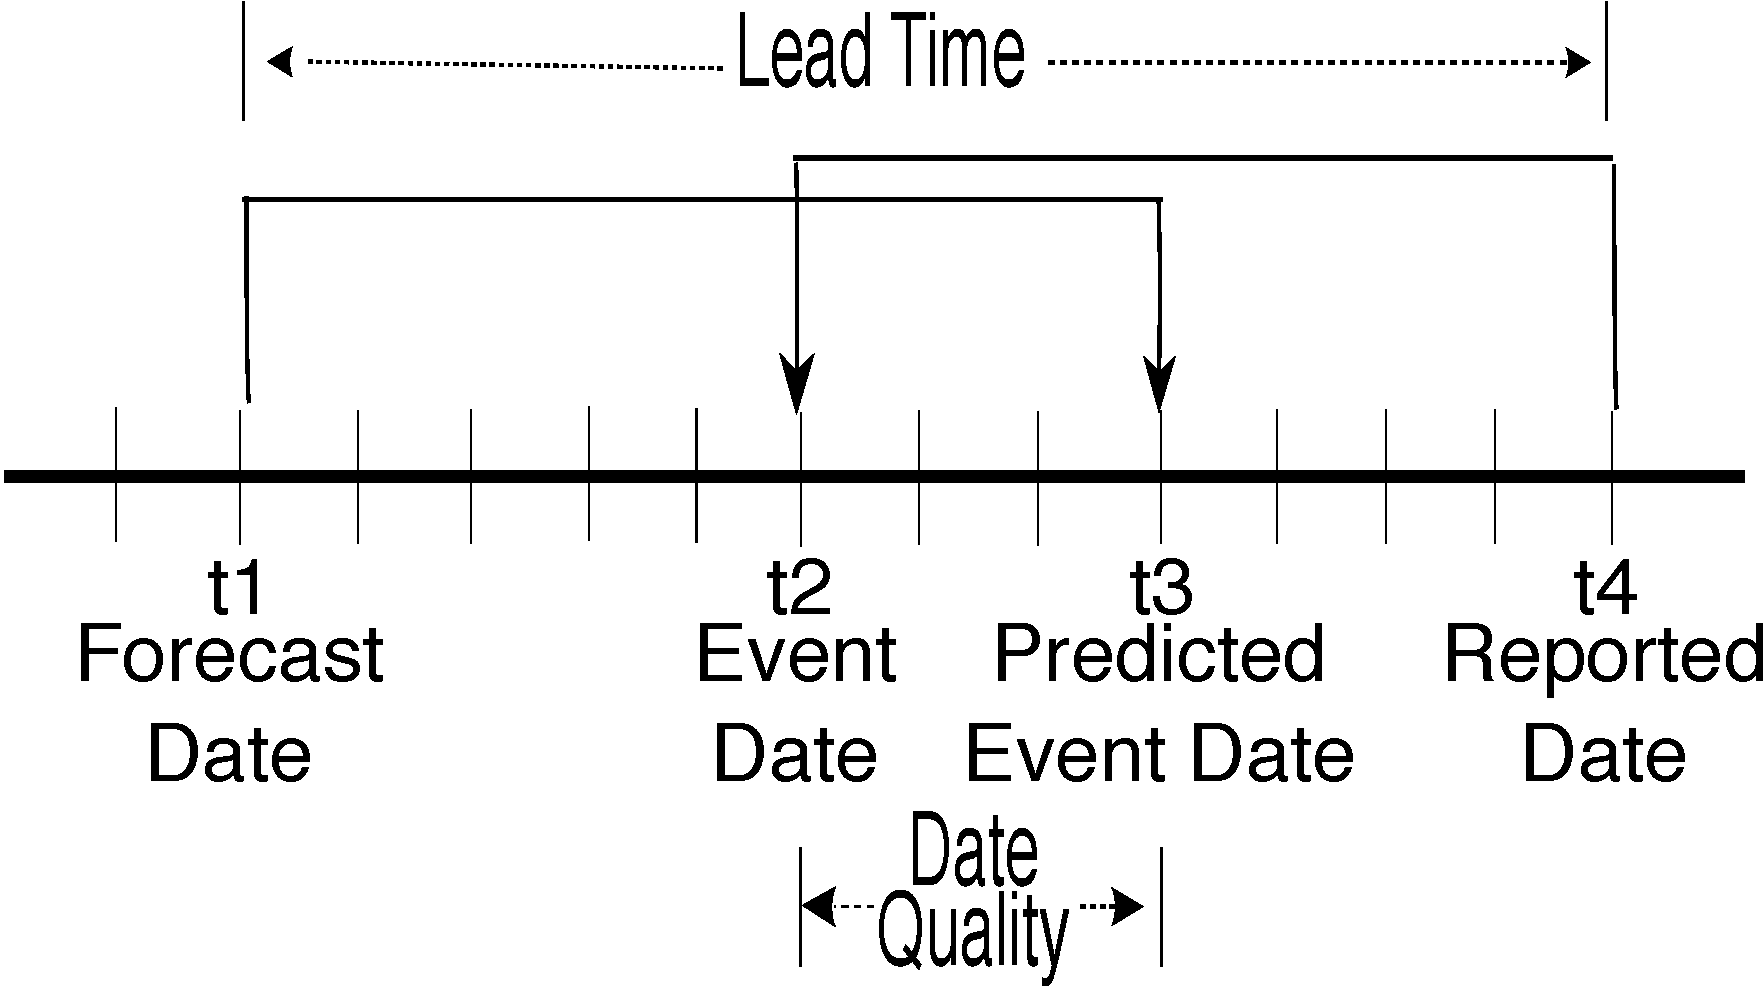
\includegraphics[width=0.5\textwidth]{timeline}
%    \caption{Matching Timeline}
%    \label{fig:timeline}
%\end{figure}


%\nocite{*}
\bibliographystyle{ieeetr}
\bibliography{references}  % sigproc.bib is the name of the Bibliography in this case
\end{document}
